\documentclass[11pt]{report}

% Geometry settings for margin
\usepackage{geometry}
\geometry{a4paper, margin=1in}  

% Fancy headers
\usepackage{fancyhdr}

% Graphics
\usepackage{graphicx}

% Hyperlinks (load last to prevent conflicts)
\usepackage{hyperref}

% Enumeration customization
\usepackage{enumitem}

% Math symbols
\usepackage{amssymb}
\usepackage{amsmath}

% Special symbols and icons
\usepackage{fontawesome}

% Multicolumn formatting
\usepackage{multicol}

% Color options
\usepackage[x11names]{xcolor}

% Tables, multirow, and arrays
\usepackage{multirow}
\usepackage{array}
\usepackage{adjustbox}

% Text boxes and highlighting
\usepackage[most]{tcolorbox}

% Option to strike through text
\usepackage{ulem}

% UTF-8 support
\usepackage[utf8]{inputenc}

% Title formatting
\usepackage{titlesec}

% Font style
\usepackage{mathptmx}  % Times New Roman-like font

% Line spacing
\usepackage{setspace}
\onehalfspacing

% Microtype for better spacing
\usepackage{microtype}

% Justification options
\usepackage{ragged2e}

% Code listings
\usepackage{listings}
\lstset{breaklines=true}

% Array package for better table formatting
\usepackage{array}

\usepackage{lineno}[switch]
\usepackage{dirtree} % For directory trees

\usepackage{longtable} %loooong looong man

\usepackage{hyperref} %linking between documents
\tcbuselibrary{breakable} %Breakin boxes


% Define simple symbols
\newcommand{\done}{\checkmark}
\newcommand{\pending}{$\square$}
\newcommand{\refine}{$\circlearrowright$}
\newcommand{\issue}{$\triangle$}
\newcommand{\draft}{\faPencil}
\newcommand{\moved}{\faArrowCircleRight}

% Custom colors
\definecolor{lightgreen}{rgb}{0.65, 0.95, 0.65}  % Slightly softer green
\definecolor{lightorange}{rgb}{1.0, 0.85, 0.65}
\definecolor{lightcoral}{rgb}{0.94, 0.6, 0.6}

\newcommand{\highlightessential}[1]{\colorbox{lightgreen}{#1}}
\newcommand{\highlightoptional}[1]{\colorbox{lightorange}{#1}}
\newcommand{\highlightrobust}[1]{\colorbox{lightcoral}{#1}}
\newcommand{\deprecated}[1]{\sout{#1}}

% Fancy headers



\title{\Huge \textbf{ONE ARM Metagenomics Pipeline}}
\author{\Large Gerald Amiel Ballena}
\date{\Large Last updated \today}

\begin{document}


	% Title page
	\maketitle
	\thispagestyle{empty}
	
	% Start main document
	\newpage



\setcounter{tocdepth}{3} 
\tableofcontents  % This generates the Table of Contents
\newpage
  % This generates the List of Figures
\newpage
\listoftables      % This generates the List of Tables
\newpage



\pagestyle{fancy}
\fancyhf{}
\fancyhead[L]{\textbf{Project Overview}}
\fancyhead[C]{\leftmark}  % Adds section title in the header
\fancyhead[R]{\thepage}

\part{Project overview}
	% Project overview in a single column
% Abstract-style tcolorbox settings
\tcbset{
	colback=gray!15,         % Light gray background
	colframe=black,          % Black border
	width=\linewidth,        % Box takes full width
	boxrule=0.5mm,           % Border thickness
	arc=0mm,                 % No rounded corners
	auto outer arc,
	fonttitle=\bfseries,     % Bold title
	coltitle=black,          % Title color
	top=0.5em,               % Add space at the top of the box
	bottom=0.5em,            % Add space at the bottom of the box
}


	
	\begin{tcolorbox}
		\raggedright
		\onehalfspacing
		\textbf{} % If you have a title, you can place it here, or leave it blank
		Metagenomic analysis of Antibiotic/Antimicrobial Resistance Genes (ARGs) in NCR (Metro Manila) hospitals, wastewaters, and surface waters.
	\end{tcolorbox}
		
\begin{tcolorbox}[title=Legend, coltitle=AntiqueWhite1]
	\begin{tabular}{p{0.45\linewidth} p{0.45\linewidth}}
		\begin{itemize}
			\item [\done] Done
			\item [\pending] Pending
			\item [\refine] Needs refinement
			\item [\issue] Unexpected issues
			\item [\draft] Drafted
			\item [\moved] Moved
		\end{itemize}
		&
		\begin{itemize}
			\item \highlightessential{Essential}
			\item \highlightoptional{Optional}
			\item \highlightrobust{Robust}
			\item \deprecated{Deprecated}
			\item TBA - needs further investigation
		\end{itemize}
	\end{tabular}
\end{tcolorbox}	
	% Two-column layout for the rest of the document



\newpage
		
\chapter{Bioinformatics Progress}

\section{Kanban Table}

\begin{longtable}{|c|p{8cm}|c|c|c|c|c|c|}
	\caption[Kanban Table]{Detailed Kanban Table for HPC and File Management Tasks} \\  % Short caption for LoT
	\hline
	\textbf{Section} & \textbf{Task} & \textbf{\pending} & \textbf{\draft} & \textbf{\refine} & \textbf{\issue} & \textbf{\moved} & \textbf{\done} \\ \hline
	\endfirsthead
	\hline
	\textbf{Section} & \textbf{Task} & \textbf{\pending} & \textbf{\draft} & \textbf{\refine} & \textbf{\issue} & \textbf{\moved} & \textbf{\done} \\ \hline
	\endhead
	
	\multirow{8}{*}{\textbf{HPC Preparation}} 
	& \highlightessential{Confirmation of Required Robustness} & & & & & & \done \\ 
	& \highlightessential{Agree upon the type of analyses} & & & & & \moved & \\ 
	& \multicolumn{7}{c|}{\textbf{SLURM request management}} \\
	& \highlightessential{Calculate using quotation from PGC} & & & & & & \done \\ 
	& \highlightessential{Setup Docker containers for SLURM} & \pending & & & & & \\
	& \highlightessential{SLURM container for simulations} & \pending & & & & & \\ 
	& \highlightoptional{Automation of SLURM requests} & \pending & & & & & \\
	& \highlightoptional{Send email for HPC usage requests} & & & \refine & & & \\ \hline
	
	\multirow{2}{*}{\textbf{File Management}} 
	& \highlightoptional{BAM file parsing} & \pending & & & & & \\
	& \highlightoptional{Interconversion between SAM and BAM} & \pending & & & & & \\ \hline
	
	\multirow{29}{*}{\textbf{Raw Read Processing}}
	& \multicolumn{7}{c|}{\textbf{Create the script}} \\
	& \highlightessential{Raw reads QC} & & & & & & \done \\ 
	& \multicolumn{7}{l}{\texttt{raw.bash}} \\ 
	& \highlightessential{Raw reads trimming} & & & & & & \done \\ 
	& \multicolumn{7}{l}{\texttt{trimmomatic.bash}} \\ 
	& \multicolumn{7}{l}{\texttt{fastp.bash}} \\
	& \highlightrobust{Looping mechanism for QC and trimming} & & & & & & \done \\
	& \multicolumn{7}{l}{\texttt{trimming-cleaning-checking.py}} \\ 
	& \highlightrobust{Data visualization} & \pending & & & & & \\
	& \highlightrobust{Determination of optimal tool/s} & \pending & & & & & \\
	& \highlightrobust{Parametric randomization} & & & & & & \done \\
	& \multicolumn{7}{l}{\texttt{trim\_randomizer.smk}} \\
	& \highlightrobust{Parse QC of all metrics in parametric randomizer} & & & & & & \done \\
	& \multicolumn{7}{l}{\texttt{parseFastQC.py}} \\
	& \highlightrobust{Determination of optimal parameters} & \pending & & & & & \\
	& \highlightrobust{Tool combination randomization script} & \pending & & & & & \\
	& \multicolumn{7}{c|}{\textbf{Test on Datasets}} \\
	& \highlightessential{Raw reads QC} & & & & & & \done \\ 
	& \highlightessential{Raw reads trimming} & & & & & & \done \\ 
	& \multicolumn{7}{l}{\texttt{\deprecated{trimmomatic.bash}}} \\ 
	& \multicolumn{7}{l}{\texttt{\deprecated{fastp.bash}}} \\
	& \multicolumn{7}{l}{\texttt{trimming-cleaning-checking.py}} \\ 
	& \highlightessential{Aggregate quality metrics} & & & & & & \done \\
	& \multicolumn{7}{l}{\texttt{summary\_stat.bash}} \\ 
	& \highlightrobust{Parametric randomization} & & & & & & \done \\
	& \highlightrobust{Parse QC of all metrics in parametric randomizer} & & & & & & \done \\
	& \multicolumn{7}{c|}{\textbf{Integrate to pipelines}} \\
	& \highlightessential{Pipeline integration of \texttt{raw.bash}} & \pending & & & & & \\
	& \highlightessential{Raw reads trimming} & & & & & & \done \\ \hline
	
	\multirow{20}{*}{\textbf{Taxonomy}} 
	& \multicolumn{7}{c|}{\textbf{Create the script}} \\
	& \highlightessential{Kraken2} & & & & & & \done \\
	& \multicolumn{7}{l}{\texttt{krakenpipeline.bash}} \\ 
	& \highlightessential{Bracken} & & & & & & \done \\
	& \multicolumn{7}{l}{\texttt{krakenpipeline.bash}} \\ 
	& \highlightessential{Diversity indices} & & & & & & \done \\
	& \multicolumn{7}{l}{\texttt{calculate\_diversity.py}} \\ 
	& \highlightoptional{MetaPhlan4} & \pending & & & & & \\ 
	& \multicolumn{7}{c|}{\textbf{Test on Datasets}} \\
	& \highlightessential{Kraken2} & & & & & & \done \\
	& \highlightessential{Bracken} & & & & & & \done \\
	& \highlightessential{Diversity indices} & & & & & & \done \\
	& \multicolumn{7}{c|}{\textbf{Integrate to pipelines}} \\
	& \highlightessential{Kraken2} & & & & & & \done \\
	& \highlightessential{Bracken} & & & & & & \done \\
	& \highlightessential{Diversity indices} & & & & & & \done \\
	& \highlightessential{Test whole pipeline} & & & & & & \done \\
	& \multicolumn{7}{l}{\texttt{metagenomics\_general.smk}} \\ 
	& \highlightrobust{Bootstrapping script} & & & & & & \done \\
	& \multicolumn{7}{l}{\texttt{bootstrapping\_rawreads.smk}} \\ \hline
	
	\multirow{18}{*}{\textbf{Assembly}} 
	& \multicolumn{7}{c|}{\textbf{Create the script}} \\
	& \highlightessential{metaSPAdes} & \pending & & & & & \\ 
	& \highlightessential{MEGAHIT} & & & & & & \done \\
	& \highlightrobust{MASURCA} & \pending & & & & & \\ 
	& \highlightrobust{PLASS} & \pending & & & & & \\ 
	& \highlightrobust{AbySS} & \pending & & & & & \\ 
	& \multicolumn{7}{c|}{\textbf{Test on Datasets}} \\
	& \highlightessential{metaSPAdes} & \pending & & & & & \\ 
	& \highlightessential{MEGAHIT} & & & & & & \done \\ 
	& \highlightrobust{MASURCA} & \pending & & & & & \\ 
	& \highlightrobust{PLASS} & \pending & & & & & \\ 
	& \highlightrobust{AbySS} & \pending & & & & & \\ 
	& \highlightrobust{\deprecated{KMA-iterative}} & \pending & & & & & \\
	& \highlightrobust{Benchmarking between all of them} & \pending & & & & & \\
	& \highlightoptional{Contig quality checking} & & \draft & & & & \\ 
	& \multicolumn{7}{c|}{\textbf{Integrate to pipelines}} \\
	& \highlightrobust{MetaWrap binning} & & & & \issue & & \\
	& \highlightessential{Kraken (MEGAHIT)} & & & & & & \done \\ \hline
	
	\multirow{4}{*}{\textbf{Binning}} 
	& \highlightoptional{Testing on datasets} & & & & \issue & & \\
	& \highlightoptional{Testing on higher depth datasets} & \pending & & & & & \\
	& \highlightrobust{Refinement of bins} & \pending & & & & & \\ 
	& \highlightrobust{Testing binning pipeline} & \pending & & & & & \\ \hline
	
	\multirow{7}{*}{\textbf{ARG Annotation}} 
	& \highlightessential{RGI} & & & \refine & & & \\ 
	& \highlightessential{ShortBRED} & & & & & & \done \\
	& \highlightoptional{AMRFinder} & & & \refine & & & \\ 
	& \multicolumn{7}{c|}{\textbf{Test on datasets}} \\
	& \highlightessential{RGI} & \pending & & & & & \\
	& \highlightessential{ShortBRED} & \pending & & & & & \\
	& \highlightoptional{AMRFinder} & \pending & & & & & \\ \hline
	
\end{longtable}


\newpage
\onecolumn
\pagestyle{fancy}
\fancyhf{}
\fancyhead[L]{\textbf{}}
\fancyhead[C]{\leftmark}  % Adds section title in the header
\fancyhead[R]{\thepage}
\section*{\centering \huge \textbf{Script Descriptions}}  % Big, bold centered title


This section covers all the scripts that were created during the Project.
\\
\\
\textit{\textbf{Listen, I’m eternally curious and I don't just want to settle for any random journal. No offense, but I’m aiming for something high-impact!}} 
\\
\\
These were created during off hours or during work hours, so some scripts might seem irrelevant at first, \textbf{\textit{but trust me, there's a conscientiousness or meticulousness to this madness.}}
\\
\\
I have separated them into folders/repositories (shameless plug here: \href{https://github.com/GABallena}{https://github.com/GABallena}) based on their relevance to the project.
\\
\\
\begin{itemize}
	\item \textbf{Project4} - Essential scripts directly related to the core analyses of the project.
	\item \textbf{Side} - Scripts that can potentially be used to increase the robustness of the paper.
	\item \textbf{Main} - Scripts related to file organization and data management, crucial for handling large datasets.
\end{itemize}



\newpage




\setcounter{section}{1}
\setcounter{subsection}{0}

% Redefine the \part command to move the title closer to the top of the page
\titleformat{\part}[display]
{\normalfont\Huge\bfseries\centering} % Title formatting
{} % No label (e.g., "Part I")
{-80pt} % This adjusts the space between the top of the page and the title. Reduce or increase this value as needed.
{\Huge} % Title font size


\pagestyle{fancy}
\fancyhf{}
\fancyhead[L]{\textbf{Project 4 scripts}}
\fancyhead[C]{\leftmark}  % Adds section title in the header
\fancyhead[R]{\thepage}


\part{Bioinformatics work}

\chapter{Project 4 Scripts}



\setcounter{section}{0}
\setcounter{subsection}{0}

\linenumbers*
\section{ARG-MGE.smk}
\begin{tcolorbox}[title=Update \dotfill \today, coltitle=AntiqueWhite1]
	Now separated into \texttt{ARG.smk} and \texttt{MGE.smk} to better modularize the workflow.
\end{tcolorbox}
\textbf{Stage: Draft}   
\textbf{General Purpose}

This pipeline is designed for \textbf{comprehensive metagenomic analysis of ARGs}, it also includes placeholders for analyses of \textbf{mobile genetic elements (MGEs)}, and \textbf{plasmid detection}. It integrates tools for \textbf{read quality control, assembly, annotation, taxonomic profiling, and structural variant (SV) detection} to provide a high-resolution view of the genetic components in metagenomic samples.
\newpage

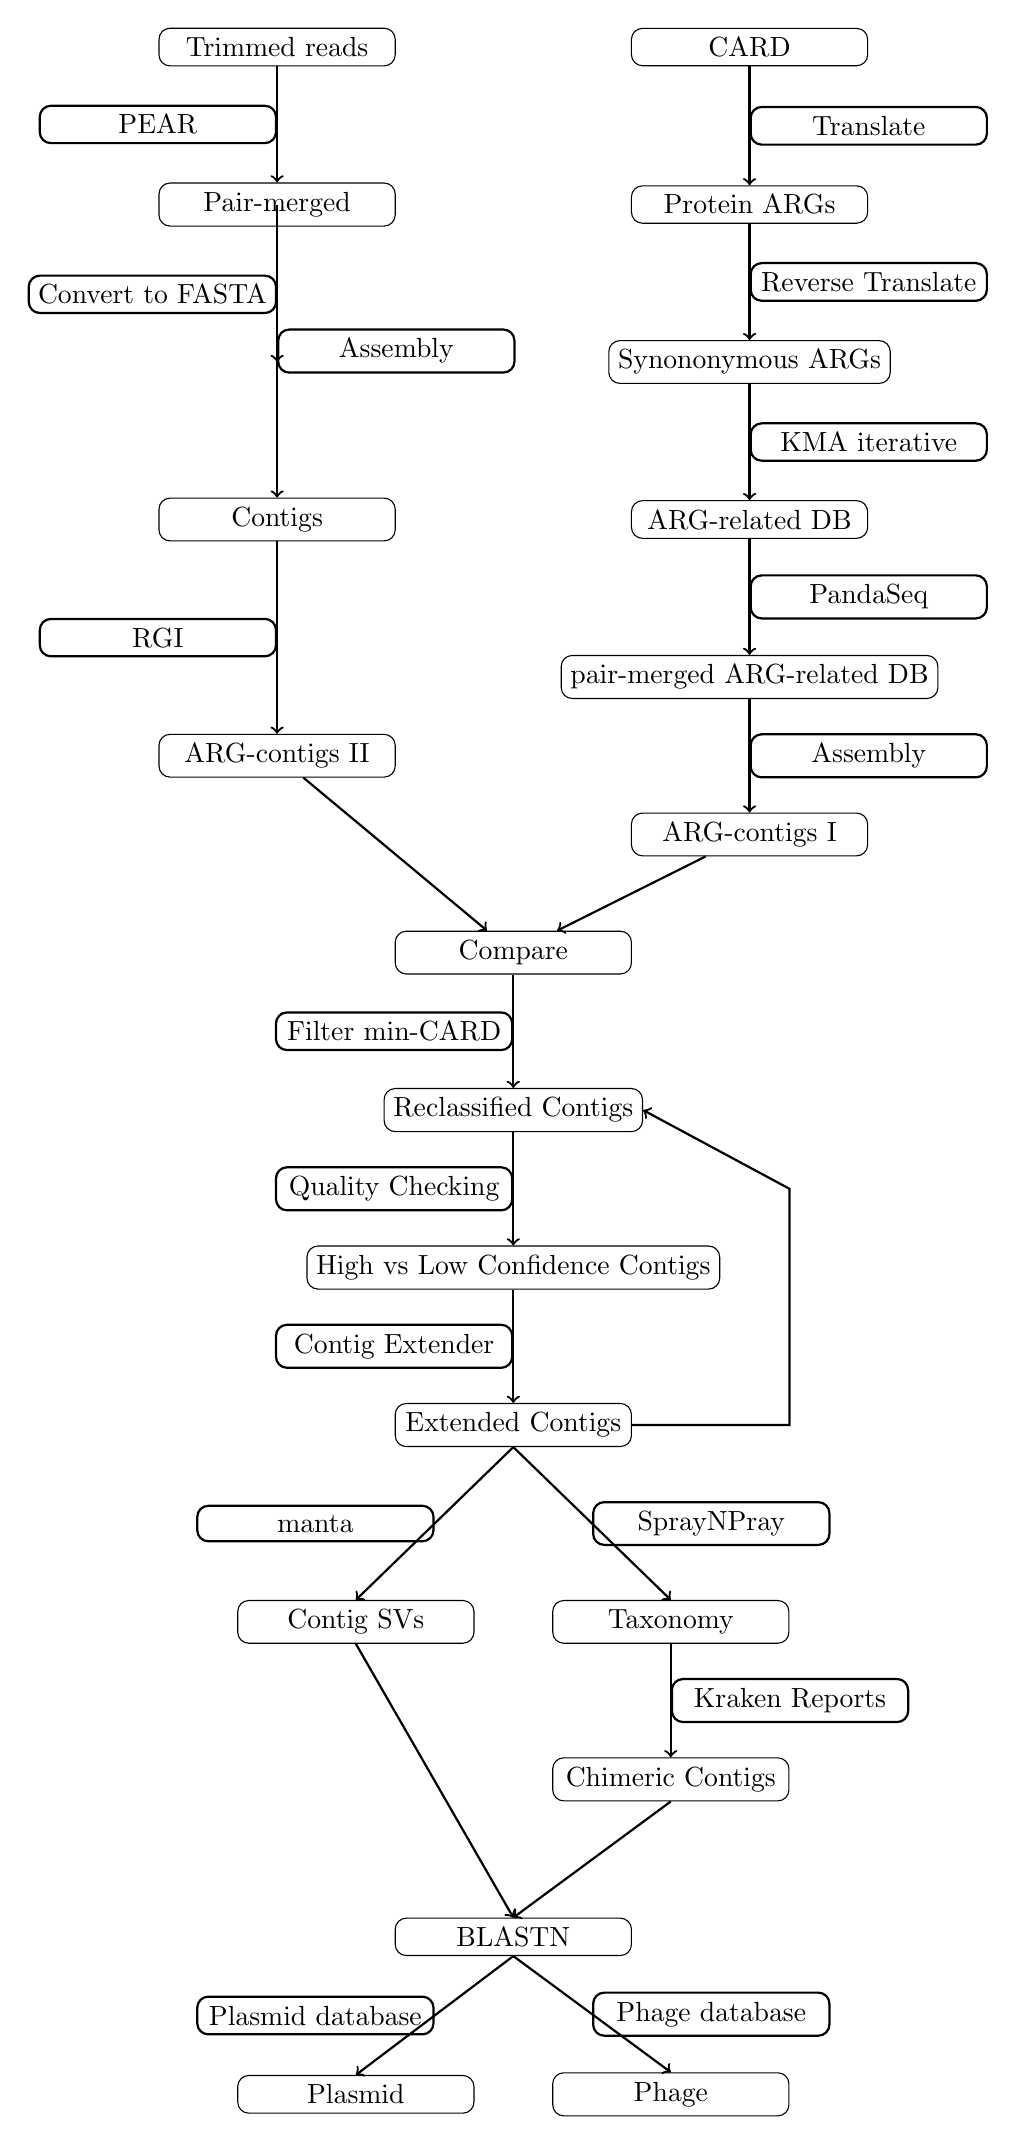
\begin{tikzpicture}[
	every node/.style={draw, rectangle, rounded corners, align=center, minimum width=3cm},
	arrow/.style={->, thick}
	]
	
	% Left side nodes
	\node (trimmedreads) at (0,0) {Trimmed reads};
	\node (pairmerged) at (0,-2) {Pair-merged};
	\node (contigs) at (0,-6) {Contigs};
	\node (argcontigs2) at (0,-9) {ARG-contigs II};
	
	% Right side nodes
	\node (card) at (6,0) {CARD};
	\node (translate) at (6,-2) {Protein ARGs};
	\node (revtranslate) at (6,-4) {Synononymous ARGs};
	\node (argrevtranslate) at (6,-6) {ARG-related DB};
	\node (pairmergedDB) at (6,-8) {pair-merged ARG-related DB};
	\node (argcontigs1) at (6,-10) {ARG-contigs I};
	
	% Middle nodes
	\node (compare) at (3,-11.5) {Compare};
	\node (reclassified) at (3,-13.5) {Reclassified Contigs};
	\node (qualitycheck) at (3,-15.5) {High vs Low Confidence Contigs};
	\node (extendedcontigs) at (3,-17.5) {Extended Contigs};
	\node (contigsv) at (1,-20) {Contig SVs};
	\node (taxonomy) at (5,-20) {Taxonomy};
	\node (chimericcontigs) at (5,-22) {Chimeric Contigs};
	\node (blastn) at (3,-24) {BLASTN};
	\node (plasmid) at (1,-26) {Plasmid};
	\node (phage) at (5,-26) {Phage};
	
	% Arrows with labels (Left Side)
	\draw[arrow] (trimmedreads) -- (pairmerged) node[midway, left] {PEAR};
	\draw[arrow] (pairmerged) -- ++(0,-2) node[midway, left] {Convert to FASTA};
	\draw[arrow] ++(0,-2) -- (contigs) node[midway, right] {Assembly};
	\draw[arrow] (contigs) -- (argcontigs2) node[midway, left] {RGI};
	
	% Arrows with labels (Right Side)
	\draw[arrow] (card) -- (translate) node[midway, right] {Translate};
	\draw[arrow] (translate) -- (revtranslate) node[midway, right] {Reverse Translate};
	\draw[arrow] (revtranslate) -- (argrevtranslate) node[midway, right] {KMA iterative};
	\draw[arrow] (argrevtranslate) -- (pairmergedDB) node[midway, right] {PandaSeq};
	\draw[arrow] (pairmergedDB) -- (argcontigs1) node[midway, right] {Assembly};
	
	% Arrows in middle
	\draw[arrow] (argcontigs2) -- (compare);
	\draw[arrow] (argcontigs1) -- (compare);
	\draw[arrow] (compare) -- (reclassified) node[midway, left] {Filter min-CARD};
	\draw[arrow] (reclassified) -- (qualitycheck) node[midway, left] {Quality Checking};
	\draw[arrow] (qualitycheck) -- (extendedcontigs) node[midway, left] {Contig Extender};
	\draw[arrow] (extendedcontigs.east) -- ++(2,0) -- ++(0,3) -- (reclassified.east);
	
	% New arrows below Extended Contigs
	\draw[arrow] (extendedcontigs.south) -- (contigsv.north) node[midway, left] {manta};
	\draw[arrow] (extendedcontigs.south) -- (taxonomy.north) node[midway, right] {SprayNPray};
	\draw[arrow] (taxonomy.south) -- (chimericcontigs.north) node[midway, right] {Kraken Reports};
	
	% Arrows to BLASTN
	\draw[arrow] (contigsv.south) -- (blastn.north);
	\draw[arrow] (chimericcontigs.south) -- (blastn.north);
	
	% Arrows from BLASTN to Plasmid and Phage
	\draw[arrow] (blastn.south) -- (plasmid.north) node[midway, left] {Plasmid database};
	\draw[arrow] (blastn.south) -- (phage.north) node[midway, right] {Phage database};
	
\end{tikzpicture}









\textbf{Preprocessing} \\
\rule{\linewidth}{0.5mm}
\subsection{Pair merging}
\textbf{Technical Notes}: \texttt{PEAR (Paired-End reAd mergeR)} compares paired-reads to correct infer the likely  bases on its associated pair\\
\textbf{Rationale}: The main goal here is to ensure good read quality for downstream analyses and to maximize the amount of data by reducing gaps in the sequence and improving confidence of base calls within that region. \texttt{seqtk} then converts compressed \texttt{FASTQ} files to \texttt{FASTA}. \\
\textbf{Rationale}\\
\textbf{Note:} Another tool, \texttt{PandaSeq} which does the same thing is used later, this usage of \texttt{PEAR} here is because it is more optimized for larger datasets - which in this case are trimmed reads.
\textbf{Note:} Conversion is necessary here as some tools cannot read FASTQ files, and instead rely on FASTA formats.

\subsection{Translation and Reverse Translation}	
\textbf{Technical Notes}: \texttt{transeq} from \texttt{EMBOSS} translates nucleotide sequences to protein sequences based on \textbf{standard genetic code}. \texttt{backtranseq} reverses this to allow iterative alignments with nucleotide sequences. \\
\textbf{Rationale}: This leverages conserved protein-level information, which is lost at the nucleotide level due to synonymous mutations - while also increasing the sensitivity to potential ARG proteins from k-mer alignment. See Nature Methods, doi: doi.org/10.1038/s41592-019-0437-4 (2019) for more details.
\\
\\
\textbf{Metagenomic Assembly} \\
\rule{\linewidth}{0.5mm}
\subsection{\deprecated{Iterative alignment of ARG-contigs}}
\textbf{Technical Notes}: \texttt{KMA} (K-mer Alignment) is used find the reverse-translated ARGs with the proximity filtering option to determine the surrounding regions of ARGs. This is done iteratively for each gene increasing the ARG-associated database. \\
\textbf{Rationale}: Firstly, \texttt{KMA} is used because, unlike \texttt{Bowtie2} and \texttt{BWA-MEM}, which were created specifically for Human metagenomics, KMA does not suffer (or suffers less) from multi-allelic databases. Secondly, iterative alignment using this process allows us to contextualize the region wherein ARGs reside - thereby narrowing our focus onto these local regions instead of looking at the global genomic context.
\textbf{Notes:} The script is designed to have a cap on the number of iterations KMA creates, increasing the database size. 

\begin{tcolorbox}[title=Sep 22 2024 Update, coltitle=AntiqueWhite1]
	This is now deprecated as there is apparently another wrapper tool called \texttt{ARG Profiler} that has a module called \texttt{ARG Extender} that literally does the same thing but with an extra filtering step that applies filters on:
		\begin{enumerate}
			\item \% query ID
			\item \% global consensus ID
			\item Mean read depth 
		\end{enumerate}
		and is thus more robust. So I will instead be using their module and cite them as such 
			\begin{verbatim}
				"This study utilized the ARGextender 
				module from ARGProfiler (Martiny, et al., 2024) 
				to extend genomic flanking regions around ARGs."
			\end{verbatim}
	\textbf{Personal Note: }\textit{Feels bad a bit on my part that someone already published the idea before I did but hey, at least I know this sort of idea is publishable haha}. Moreover, it does save us time because I only have to \texttt{copy-paste} their module (and associated scripts) into the existing pipeline.

\end{tcolorbox}

	
\subsection{Merging of paired reads}
\textbf{Technical Notes}: \texttt{PANDASeq} is then used to further refine the paired-reads collated in the ARG-related genes database. \\
\textbf{Rationale}: \texttt{PANDASeq} was chosen as, while being slower than \texttt{PEAR}, it is more accurate. This mergins step is included to ensure that only high-confidence reads are assembled. 
\textbf{Note:} We leverage the fact that the ARG-related genes database is smaller compared to the raw metagenomic reads database.
	
\subsection{Guided Metagenomic Assembly}
\textbf{Technical Notes}: \texttt{metaSPAdes} is then used to create contiguous sequences from these local regions by extending them using reads from the whole metagenomic pool. Additionally, Contigs are filtered by length here to remove possible artefacts. \\
\textbf{Rationale}: \texttt{metaSPAdes} was chosen as, while being slower than \texttt{MEGAHIT}, it is optimized in handling highly diverse and mixed microbial populations. CARD is used here because it is manually curated and updated regularly - in order to be included in the database, there must be clinical data (e.g. ASTs(Antimicrobial susceptibility testing)) involved in the study.
\\	 \textbf{Notably, this would decrease the sensitivity of our ARGs - and would mostly be biased towards those reported in the clinical setting}. To counter this, we could also incorporate other tools such as \texttt{ResFinder}, the \texttt{NCBI AMR Database}, and \texttt{ARG-ANNOT}
\\	\textbf{Notes:} Filtering of contig length is handled by a python script called \texttt{minimum\_length\_CARD.py}.
\\	\textbf{Notes:} Contigs are further extended using contigextender to form scaffolds 
\\	\textbf{Notes:} Might add other contig extendending programs like \texttt{GapFiller} - which leverages mate-pair information 
\\
\\
\textbf{Contig Quality Checks} \\
\rule{\linewidth}{0.5mm}
	
\subsection{Confirmation of contigs with ARGs}
\textbf{Technical Notes}: \texttt{RGI} scan the contigs and check whether which contigs created by \texttt{metaSPAdes} have ARGs in them. \\
\textbf{Rationale}: \texttt{metaSPAdes} may have created contigs that DO NOT contain ARGs, and have instead assembled them into a more matching contig (a false-positive misassembly) - this can happen because of the different databases being used; also parallelization of methods like this increases robustness because it has been confirmed independently from different starting points (bottom-up vs top-down approach). This allows us to filter ARG-containing contigs. \\
\textbf{Notes:} \texttt{RGI} is the official scanner of \texttt{CARD}.



\subsection{Standard Contig Quality Metrics}
\textbf{Technical Notes}:A custom \texttt{Python} script \texttt{calculate\_contig\_quality.py} is created to do another round of checking contig quality for downstream analysis, \texttt{R} scripts (TBA) are used to visualize the data. \\
\textbf{Notes}: The \texttt{Python} script will measure standard contig quality metrics: N50, L50, GC-content, and coverage, as well as more robust metrics: N90 and L90.


\subsection{Read-mapping}
\textbf{Technical Notes}: \texttt{Samtools} is used here to map the raw reads from the larger database back to the assembled contigs and then calculates the coverage over the entire contig. \\
\textbf{Rationale}: Read-mapping is a quality control protocol used in metagenomics, to determine the quality of the assembly. High-coverage means that many of the k-mers align well with that region of the contig, while low coverage is evidence of inconsistent mapping and that the contigs should be refined, split, or discarded.\\
\textbf{Note} If there are persistent (after further refinement and reassemblies) sudden differences in coverage across a contig, that contig could be chimeric, meaning, it could be from two different populations. 
\\ \textbf{Extra note} A \texttt{Python} script \texttt{plot\_and\_detect\_intermediate\_coverage.py} is included in the pipeline that is determine visualize and check how the coverage changes over contig regions. In general, they could be interpreted as the following:
\begin{enumerate}
	\item \textbf{Smooth, Uniform Coverage}: Typically shown by well-assembled contigs.
	\item \textbf{Sharp Coverage Drop}: May need to be split or flagged for reassembly. May also be a misassembly point (chimeric contig) or caused by a structural variant.
	\item \textbf{Coverage Gaps}: Regions with little to no read support; a strong indicator of misassembly.
	\item \textbf{Gradual Drops}: Overlapping reads, repetitive or duplicate regions, partial HGT, sequence heterogeneity, or coverage differences due to a mixed population. Repeats and duplications can be filtered out using tools like \texttt{RepeatMasker} or \texttt{BLAST} (TBA).
	\item \textbf{Sharp Increase}: May be due to repetitive or duplicated regions, amplification bias from PCR, HGT, SV, chimeras.
\end{enumerate}


\subsubsection{Read mapping parameters}
\textbf{Technical Notes}: Four (4) Tools will be used in parallel to do the read mapping process \texttt{BWA} \texttt{Bowtie} \texttt{KMA}, and \texttt{minimap2}, their parameters have been adjusted to map reads at 95 \% identity to the contigs.
	
\begin{table}[h!]
	\centering
	\begin{adjustbox}{max width=\linewidth}
		\begin{tabular}{|p{3cm}|p{3cm}|p{3cm}|p{3cm}|p{3cm}|}
			\hline
			\textbf{Mapper} & \textbf{K-mer Length} & \textbf{Mismatch Penalty} & \textbf{Gap Opening Penalty} & \textbf{Gap Extension Penalty} \\ \hline
			\texttt{BWA} & 21 & 5 & 7 & 2 \\ \hline
			\texttt{BWA} & 31 & 4 & 6 & 2 \\ \hline
			\texttt{BWA} & 51 & 3 & 5 & 1 \\ \hline
			\texttt{Bowtie2} & - & 4,2 & 5,2 & 5,2 \\ \hline
			\texttt{KMA} & Default & 95\% identity & Automatic & Automatic \\ \hline
			\texttt{Minimap2} & - & 5 & 7,2 & 4,1 \\ \hline
		\end{tabular}
	\end{adjustbox}
	\caption{Example table of mapper configurations without command example}
	\label{tab:mapper_configurations}
\end{table} 
\textbf{Rationale}: 95 \% identity is used to increase sensitivity - as is standard for determining homologous sequences. This adjustment was made because k-mers are either attach or don't. Parallelization is used to increase robusness.\\
\textbf{Note} K-mer extension is used to increase the accuracy of mapping. \texttt{BWA} k-mer lengths can be adjusted, while \texttt{KMA} does it by default. The others, cannot be adjusted. \\
	% Then within your document:
\tcbset{
	colback=lightgray!30, colframe=black, 
	width=\linewidth, boxrule=0.5mm,
	arc=2mm, auto outer arc,
	fonttitle=\bfseries
}

	\begin{tcolorbox}[title=Note, coltitle=white]
		I chose to change the script to not allow gaps during this phase as we already used reverse translation earlier to correct for synonymous codons, and protein sequences are more important when it comes to ARG function, the new values are below. I also added protein-based read mapping. 
	\end{tcolorbox}


\begin{table}[h!]
	\centering
	\begin{adjustbox}{max width=\linewidth}
		\begin{tabular}{|p{2.5cm}|p{2.5cm}|p{2.5cm}|p{2.5cm}|p{2.5cm}|}
			\hline
			\textbf{Tool} & \textbf{K-mer Length} & \textbf{Mismatch Penalty} & \textbf{Gap Opening Penalty} & \textbf{Gap Extension Penalty} \\ \hline
			\texttt{BWA} & 21, 31, 51 & 5, 4, 3 & 1000 & 1000 \\ \hline
			\texttt{Bowtie2} & - & 4,2 & 1000,1000 & 1000,1000 \\ \hline
			\texttt{KMA} & - & 95\% identity & Automatic & Automatic \\ \hline
			\texttt{Minimap2} & - & 5 & 1000,1000 & 1000,1000 \\ \hline
		\end{tabular}
	\end{adjustbox}
	\caption{Alignment parameters for ungapped alignments across \texttt{BWA}, \texttt{Bowtie2}, \texttt{KMA}, and \texttt{Minimap2}}
	\label{tab:alignment_parameters}
\end{table}
	
	
\begin{table}[h!]
	\centering
	\begin{adjustbox}{max width=\linewidth}
		\begin{tabular}{|p{3cm}|p{4cm}|p{5cm}|}
			\hline
			\textbf{Tool} & \textbf{Input Files} & \textbf{Key Parameters} \\ \hline
			\textbf{tblastn} & 
			\begin{itemize}
				\item Protein sequences: \texttt{Translated protein sequences contigs}
				\item Nucleotide database: \texttt{Cleaned sequence database}
			\end{itemize} 
			& 
			\begin{itemize}
				\item \texttt{-outfmt 6}
				\item \texttt{-evalue 1e-5}
				\item \texttt{-gapopen 5}
				\item \texttt{-gapextend 2}
				\item \texttt{-matrix \texttt{BLOSUM62}}
			\end{itemize} \\ \hline
			
			\textbf{blastp} & 
			\begin{itemize}
				\item Protein sequences: \texttt{Translated protein sequences contigs}
				\item Protein database: \texttt{Translated cleaned sequence database}
			\end{itemize} 
			& 
			\begin{itemize}
				\item \texttt{-outfmt 6}
				\item \texttt{-evalue 1e-5}
				\item \texttt{-gapopen 5}
				\item \texttt{-gapextend 2}
				\item \texttt{-matrix \texttt{BLOSUM62}}
			\end{itemize} \\ \hline
			
		\end{tabular}
	\end{adjustbox}
	\caption{Protein read-mapping parameters for \texttt{tblastn} and \texttt{blastp}}
	\label{tab:protein_read_mapping}
	
\end{table}

\textbf{Rationale}: The main rationale for adding a protein-based read mapping protocol is because ARGs are primarily about their \textit{\textbf{protein-protein interactions}} (biological relevance). This method also accounts for frameshifts with higher specificity to homologous regions. \\
\textbf{On a personal note}: This approach may also require further exploration into whether protein-protein interactions are altered—perhaps by investigating changes in binding sites. Which is a story for another day (\textit{\textbf{why do I do this to myself?}})

\subsection{Taxonomic profiling of reads and contigs}
\textbf{Technical Notes}: \texttt{Kraken2} uses k-mer-based classification to assign taxonomy based on raw-reads. While \texttt{SprayNPray} complements this by assigning taxonomy at the contig level. \\
\textbf{Rationale}: By comparing their respective databases with our ARG-related databases, we will be able to connect our reads and/or contigs to their corresponding taxa, uncovering the microbial hosts responsible for carrying and potentially spreading ARGs in the environment.

\subsection{Detect structural variants (SVs) in contigs}
\textbf{Technical Notes}: \texttt{Manta} identifies large genomic rearrangements such as insertions, deletions, and duplications. \\
\textbf{Rationale}: Chimeric contigs may be due to systematic error or real biological signals. These chimeric contigs can be detected by \texttt{Kraken2} and \texttt{SprayNPray} (i.e., when a portion of a contig is being assigned to different taxa). The rationale behind this step is to investigate whether structural variations are present — which may be evidence of horizontal gene transfer (HGT) events.

\subsection{Sketching contigs followed by calculating \texttt{Bray-Curtis} diversity}
\textbf{Technical Notes}: \texttt{Mash Sketch} uses a MinHash approach to generate a presence/absence profile of ARGs across contigs. This gives us a quick snapshot of what the contigs “look like” in terms of ARG content. For \texttt{Bray-Curtis} diversity, we calculate a dissimilarity matrix from the abundance data of ARGs, followed by a PCoA plot to visualize similarities between contigs based on their ARG profiles. \\
\textbf{Rationale}: The \texttt{Mash Sketch} helps rapidly identify the genetic makeup of contigs in terms of ARGs, which provides a foundation for further investigation. By applying \texttt{Bray-Curtis} diversity and using PCoA, we can group contigs based on their ARG similarity. If contigs with the same sketch group together, we can trace them back to their taxonomic IDs to identify the microbial hosts. However, if contigs have similar ARG profiles but belong to different taxa, this could serve as \textbf{evidence for \textbf{Horizontal Gene Transfer (HGT)}}. This dual approach allows us to trace ARG spread and potential HGT events in a metagenomic context. \\
\textbf{Note}: \texttt{Bray-Curtis} (dis-)similarity is most often used as a presence or absence diversity metric.
\\
\\ 
\textbf{Transposition} \\
\rule{\linewidth}{0.5mm}

\section{MGE.smk}

\subsection{Determination of Transposons (TBA)}
\textbf{Technical Notes}: Tools such as the following can be used:
\begin{itemize}
	\item \texttt{HMMER3} suite
	\item \texttt{Tnppred} - a transposon predictor tool
\end{itemize}

\textbf{Rationale}:  % The rationale here should be filled in with relevant details.
\\
\\ 
\textbf{Plasmids} \\
\rule{\linewidth}{0.5mm}

\subsection{Determination of putative plasmids}
\textbf{Technical Notes}: The tools listed below will be used in parallel. Plasmids are considered valid when all 4 tools predict plasmid signatures in the contig.
\begin{itemize}
	\item \texttt{PlasPredict} pipeline
	\item \texttt{Recycler}
	\item \texttt{PlasmidFinder}
	\item \texttt{MOBSuite} plasmid marker annotator
\end{itemize}
If plasmid signatures are present, \texttt{plasmidSPAdes} along with \texttt{GapFiller} will be used to check if the contig can circularize. \texttt{oriTfinder} will then be applied to contigs with fewer than 4 fragments. A \texttt{Python} script (TBA) will calculate GC skews of the chimeric contig and compare it to its taxonomic counterparts. Another \texttt{Python} script (TBA) will normalize the data according to \texttt{16S rRNA} from trimmed reads. Lastly, plasmid percentage will be calculated based on reads mapped to putative plasmids over the total reads. A code snippet is present called \texttt{calculate\_plasmid\_percentage.py}.

\textbf{Equation}:
\[
\text{Plasmid Percentage} = \left( \frac{\text{Plasmid Reads}}{\text{Total Reads}} \right) \times 100
\]

\textbf{Rationale}: \texttt{oriTfinder} looks for \texttt{origin of transfer} sites (\texttt{oriT}), which are characteristics of conjugative plasmid . This whole sub-pipeline is to look for evidence of conjugative plasmid transfer as the cause of these chimeric contigs. Normalization and percentage counts are used here to further check whether these "plasmids" align with our understanding of the average plasmid copy number. \\
\textbf{Note}: Will also be drafting a script (TBA) to do sliding window analysis of \texttt{GC-skews} - as different characteristics of this curve can be interpreted in different ways. \\
\\ 
\textbf{Phages} \\
\rule{\linewidth}{0.5mm}	
	
\subsection{Phage influence signatures}
\textbf{Technical Notes}: They will be determined using a variety of tools:\\
After prediction with \texttt{Prodigal}, a sequence was considered a phage if it was identified by two-thirds (2/3) of the program stated below: 
\begin{itemize}
	\item \texttt{VirSorter}: Identifies viral signatures within microbial genomes and separates prophages from bacterial sequences.
	\item \texttt{PHASTER}: A web-based tool for phage search and annotation, identifying integrated prophages.
	\item \texttt{VIBRANT}: A tool that combines several approaches to identify and annotate phage elements in metagenomic sequences.
\end{itemize}
\textbf{Rationale}:This analysis aims to detect potential phage signatures in the chimeric contigs. Since phages are mobile genetic elements, their involvement in transferring ARGs through transduction is highly relevant.Phages, especially temperate phages, can integrate into bacterial genomes and excise themselves, sometimes carrying host genetic material, such as ARGs, with them.The integration and excision signatures detected in contigs will provide evidence of possible transduction events in our datasets, supporting the hypothesis of ARG dissemination via phages.

\subsection{Annotion of Phage genes (TBA)} 
\textbf{Technical Notes} All these proteins will be queried against the following databases.
\begin{enumerate}
	\item \texttt{{PFAM}}
	\item \texttt{VOGdb}
	\item \texttt{eggNOG} 
\end{enumerate}
Using a combination of \texttt{eggNOG-mapper(mapper.py)} and \texttt{HMMER} with the following thresholds: E-value $<$ 10\textsuperscript{-5}, score $\geq$ 50. \texttt{Active} prophages were then separated from \texttt{Inactive} ones using the tool \href{https://github.com/WenchenSONG/Prophage-Hunter}{\texttt{Prophage Hunter}} -- default scoring parameters. Results were considered false-positives if they were considered active by \texttt{Prophage Hunter} but were 'not phage' for \texttt{VirFinder} and \texttt{MetaPhinder} as \href{https://academic.oup.com/nar/article/47/W1/W74/5494712}{previously done by the authors of the tool.} HMM profiles were downloaded from \href{https://promge.embl.de/download.cgi}{proMGE database -- which are calibrated to different recombinases: (huh\_y1, huh\_y2, ser\_tn, ser\_ce, ser\_lsr, cas1)} and used against the putative recombinases to further divide them into distinct categories. To determine whether these genes are of viral or bacterial origin, \href{https://www.nature.com/articles/s41587-020-00774-7}{\texttt{CheckV} was used}.
\\ \textbf{Rationale}
\\ \textbf{Notes}


\subsection{Phage Signature Extraction and Phylogenetic Analysis}
\textbf{Technical Notes}: Phage-associated genes will be extracted from the chimeric contigs, followed by phylogenetic analysis to uncover evolutionary relationships. \texttt{FastTree} will be used to build a phylogenetic tree based on the extracted phage genes. For visualization, tools like \texttt{iTOL} or \texttt{FigTree} can be used to generate an interpretable phylogenetic tree.

\noindent \textbf{Rationale}: Phage genes embedded in chimeric contigs (their taxonomy) may serve as strong evidence of horizontal gene transfer (HGT) events. The aim here is to check the evolutionary origins of the phage genes found in our dataset and their potential involvement in the dissemination of ARGs.

\subsection{Directory tree}
\textbf{Notes:} The final directory tree should look like this to help you visualize. \textbf{Notice the multiple \texttt{path/to/} here as this is still (WIP)}:

\dirtree{%
	.1 /project\_root/.
	.2 path/to/cleaned\_reads/ \DTcomment{Prerequisite}.
	.2 path/to/merged\_reads/.
	.2 path/to/CARD\_db/ \DTcomment{Prerequisite - Database}.
	.2 path/to/output/.
	.3 final\_annotated\_plasmids.fasta.
	.3 fpkm\_normalized\_plasmids.txt.
	.3 categorized\_MGEs.txt.
	.3 final\_filtered\_contigs.fasta.
	.2 path/to/logs/.
	.3 predict\_plasmids.log.
	.3 run\_mob\_suite.log.
	.3 check\_plasmidfinder.log.
	.3 calculate\_gc\_skew.log.
	.2 path/to/plaspredict\_output/.
	.2 path/to/PFAM\_db/ \DTcomment{Prerequisite - Database}.
	.2 path/to/TnpPred\_db/ \DTcomment{Prerequisite - Database}.
	.2 path/to/plasmid\_prediction/.
	.3 predicted\_plasmids.fasta.
	.3 plasmidfinder\_report.txt.
	.3 oritfinder\_report.txt.
	.3 tnpred\_report.txt.
	.2 path/to/plasmidspades\_output/.
	.3 plasmid\_assembly.fasta.
	.2 path/to/mob\_suite\_output/.
	.3 mob\_suite\_summary.txt.
	.2 path/to/gc\_skew\_analysis/.
	.3 gc\_skew\_plot.png.
	.2 path/to/read\_mapping/.
	.3 reads\_mapped\_to\_plasmids.bam.
	.3 plasmid\_read\_count.txt.
	.3 total\_read\_count.txt.
}







\rule{\linewidth}{0.5mm}
\textbf{Homework?} 
\subsection{Future Considerations}
Will continue improving this section (everything regarding HGT) by evaluating the results from these tools, aligning them with ARG presence, and refining the approach for identifying conjugation, transposon, and transduction events within chimeric contigs. This may also involve validating phage activity—\textit{again, why do I do this to myself?}


\newpage
\linenumbers*
\section{metagenomics\_general.smk}
\textbf{Stage: Done} \\   
\textbf{General Purpose taxo-metagenomics}\\
\textbf{Specifics:}This pipeline is designed for \textbf{The essentials in metagenomics}, which includes \textbf{quality checking, filtering, and trimming of raw reads to clean reads}. As well as the usual \textbf{taxo-metagenomic analysis}. 


\subsection{Quality control (Pre-processing)}		

\textbf{Raw trimming of raw metagenomic data} 
\\ \textbf{Technical Notes}: \texttt{FastQC} is used on \textbf{raw reads}
\\ \textbf{Rationale}: This is mainly used as a point of comparison - determine whether the next step (trimming) was effective. This pre-processing step is the starting point in any and all metagenomics pipelines. 
\\ \textbf{Notes}: This whole quality control steps are interconnected with each other. 
\subsection{Trimming} 
\textbf{Technical Notes}: \texttt{Trimmomatic} is used on \textbf{raw reads}
\\ \textbf{Rationale}: Trimming involves removing low quality bases (often depending on something called the Phred Score - which is just a measure of how "confident" we are that the base on that site was accurate), adapters, and filtering reads that go below a specific length threshold. 
\\ \textbf{Notes}: Journals often report the parameters on \texttt{Trimmomatic} (or any trimmer they decide to use); this is often so that the study is reproducible, should one decide to actually reproduce the study starting from scratch (raw reads). 
\\ \textbf{Notes}: There are many different trimmers each with their own strengths and weaknesses, \texttt{Trimmomatic} is just the most popular trimmer and is thus used here, though studies differ in the parameters they used for trimming - which often dictates how strict they are with what they define as "good enough". \\
\\ \textbf{Perspective}: Why different people choose different trimmers depend on the \textbf{strengths and weaknesses} of the trimmer e.g. trimmers like "fastp" is used because it's fast making it suitable for very large datasets like deep sequencing. While some trimmers like \texttt{Sickle} has automatic adjustment over the entire sequence - which makes it useful for very ancient datasets where DNA is often highly-degraded. Other times, it's for \textbf{convenience} like \texttt{Trim-Galore} which combines \texttt{FastQC} and \texttt{Cutadapt} trimmer in a single command. Another good example is \texttt{BBDuk} which is part of a larger package called \texttt{BBtools}, \texttt{BBDuk} also has an built-in contamination detection - so it's particularly good at filtering out usual contaminants like sequences known to be from the human genome. so you can simply just use all the modules in that package for all-in-one processing.  Other times, it's just \textbf{familiarity}. 
\\\\
\textbf{Quality checks of post-trimmed data} 
\\ \textbf{Technical Notes}: \texttt{FastQC} is used on \textbf{trimmed reads} to determine how effective the trimming process was. 
\\ \textbf{Rationale}: If the trimming process was effective, we should notice a better quality reads here, otherwise, we might have to adjust the trimming parameters. 
\\ \textbf{Notes}: Determination of whether the trimmed reads are "clean enough" is more of an art rather than actual science, though thresholds exist like Phred $>$ 20 or Phred $>$ 30 depending on how strict you are as a researcher. 
\\
\\
\\ 
\textbf{Processing cleaned reads} \\
\rule{\linewidth}{0.5mm}
\subsection{Metagenomic Taxonomy}	
\textbf{Taxonomy from Cleaned Reads} 
\\ \textbf{Technical Notes}: \texttt{Kraken2} is used on \textbf{raw reads} to determine which species they came from. 
\\ \textbf{Rationale}: Taxonomy based on reads is standard on metagenomics instead of using assembled contigs because information is lost during the assembly process. By using cleaned reads we make sure that: 
	 \begin{enumerate}
	 	\item We are maximizing the amount of data
	 	\item We are not being biased by low quality reads
	 \end{enumerate}
\textbf{Notes}: There are many ways in which taxonomy is assigned to raw reads the \texttt{Kraken-based} packages use a curated database that links k-mers from your database to k-mers generated from their database (usually manually curated).  
\\ \textbf{Notes}: Others like \texttt{MetaPhlan} first create "markers" that are based off of known sequences, and then scan your raw reads for these markers, which it then checks for under what taxon/taxa that marker fell under. \\

\subsection{Diversity analysis}	
\textbf{Diversity analysis per site or sample} 
\\ \textbf{Technical Notes}: Here \texttt{Bracken} - an extension of the \texttt{Kraken} packages or \texttt{Qiime2} are often used to calculate diversity. Instead I opted to create my own \texttt{Python} script \texttt{calculate\_diversity.py} because:
	 \begin{enumerate}
	\item I find that the diversity indices in either tools are limited to only the most often used i.e. the most popular indices - so it is not comprehensive
	\item I've had problems integrating them into the pipeline because some dependency limitations, un-updated scripts, and a pre-processing step that requires converting all of \texttt{Kraken2, Bracken} files, then importing them to \texttt{Qimme2} which is too time-consuming and inefficient - my script just automatically calulates from \texttt{Bracken} outputs and just puts out all the possible (non-phylogenetic-based-which you would need a phylogenetic tree to build first) indices out there.  
	\end{enumerate}
\textbf{Rationale}: Taxonomy based on reads is standard on metagenomics instead of using assembled contigs because information is lost during the assembly process. By using cleaned reads we make sure that: 
\begin{enumerate}
	\item We are maximizing the amount of data
	\item We are not being biased by low quality reads
\end{enumerate}
\textbf{Notes}: There are many ways in which taxonomy is assigned to raw reads the \texttt{Kraken-based} packages use a curated database that links k-mers from your database to k-mers generated from their database (usually manually curated).  
\\ \textbf{Notes}: Others like \texttt{MetaPhlan4} first create "markers" that are based off of known sequences, and then scan your raw reads for these markers, which it then checks for under what taxon/taxa that marker fell under. 

\subsection{Directory tree}
\dirtree{%
	.1 /project\_root/.
	.2 configs/.
	.3 config.yaml.
	.2 path/to/raw\_reads\_dir/ \DTcomment{Prerequisite - Raw Data}.
	.3 sample1\_R1.fastq.gz.
	.3 sample1\_R2.fastq.gz.
	.3 sample2\_R1.fastq.gz.
	.3 sample2\_R2.fastq.gz.
	.2 path/to/trimmed\_reads\_dir/ \DTcomment{Prerequisite - Trimmed Data}.
	.3 sample1\_R1\_paired.fastq.gz.
	.3 sample1\_R2\_paired.fastq.gz.
	.3 sample2\_R1\_paired.fastq.gz.
	.3 sample2\_R2\_paired.fastq.gz.
	.2 path/to/fastqc\_output\_dir/.
	.2 path/to/kraken\_output\_dir/.
	.3 sample1.k2report.
	.3 sample1.kraken2.
	.3 sample2.k2report.
	.3 sample2.kraken2.
	.2 path/to/bracken\_output\_dir/.
	.3 sample1.bracken.
	.3 sample1.breport.
	.3 sample2.bracken.
	.3 sample2.breport.
	.2 path/to/cleaning\_results\_dir/.
	.3 summary\_report.txt.
	.2 logs/.
	.3 calculate\_diversity.log.
	.2 path/to/output/.
	.3 diversity\_matrices.tsv.
}


\newpage
\linenumbers*
\section{trim\_randomizer.smk}
\textbf{Stage: Done}   \\
\textbf{Purpose: Randomization of trimming parameters}

This is a module that will be part of a bigger pipeline. The idea here to is randomize parameters in a variety of trimmers in this case \texttt{Trimmomatic},
\texttt{fastp}, \texttt{CutAdapt}, \texttt{BBDuk}, and \texttt{Sickle} - famous bioinformatics trimming tools. \texttt{Trimmomatic} and \texttt{Sickle} in particular are widely used in \texttt{Illumina}-based data.\\ 

\subsection{Random Parameter Generation}
\textbf{Technical Notes}: Random parameters are generated for each trimming tool (Trimmomatic, Fastp, Cutadapt, BBDuk, Sickle). This is done using the \texttt{random module}, which creates random values for parameters such as quality scores, read length, adapter sequences, and error rates. These parameters are stored in the \texttt{generated\_parameters} dictionary to ensure consistency across iterations for each sample.\\
\textbf{Rationale}:By randomizing parameters, the workflow allows for testing different parameter sets across multiple iterations to find optimal settings for trimming and quality control.
\\ \textbf{Notes}: This approach helps with parameter exploration, particularly when you are unsure which trimming settings will give the best results. The randomness provides variability, which can highlight which parameters consistently lead to good results.

\subsection{Log Parameters to a \texttt{TSV} File}
\textbf{Technical Notes}: Each set of generated parameters is logged into a separate TSV file (e.g., \texttt{trimmomatic\_params.tsv}, \texttt{fastp\_params.tsv}). The file headers are written only once, and parameters are appended as the trimming steps proceed. This is done in a structured way so that you can track the exact parameters used for each sample and iteration.\\
\textbf{Rationale}:Logging ensures reproducibility and transparency in bioinformatics workflows. Having a record of all the parameter values used in each iteration is crucial for comparing results and for future reference
\\ \textbf{Notes}: This practice is a standard in scientific workflows where random parameter generation is involved. It helps maintain a clear audit trail of the steps performed and aids in troubleshooting or refining workflows later.

\subsection{Define \texttt{Rules} for Each Tool}
\textbf{Technical Notes}: The script uses \texttt{Snakemake rules} to define separate rules for each tool which include
	\begin{enumerate}
		\item Input folder (as the script is designed to go through all the \texttt{FASTQ} samples within the folder)
		\item Output folder, where the processed files will be saved (e.g., trimmed paired and unpaired reads). The script is designed to keep all the \texttt{trimmed reads} in separate files. 
		\item Params: Fetches the parameters to be randomized. 
	\end{enumerate} 
\textbf{Rationale}:Using Snakemake here allows for parallel execution of the workflow. This parallelization if very important as the generation of random paramaters is created using a random \texttt{seed}. Using a random \texttt{seed} like this allows us to replicate what the parameters that had the optimal results were by tracking down what seed was assigned as dictated in the \texttt{TSV} file.\\
\textbf{Note} keep in mind that this will create a large number of folders if you decide to iterate many times - as each iteration, per tool, will have its own folder full of trimmed reads, per sample/site.

\subsection{Interpretation and Analysis of Results (TBA)}
\textbf{Technical Notes}: Once all iterations have completed, the trimmed files can be analyzed to determine which parameters led to the best results in terms of quality and length distribution of reads. There are many different metrics that can be used to interpret the results, including (but not limited to)
\begin{enumerate}
	\item Quality Scores - significant differences in quality among sites and across entire sequences (Phred score, Contamination, Adapter Removal, N Content, Length Distribution, etc.). Can be done using tools like \texttt{FastQC}
	\item Visualization can be done using \texttt{Rstudio} or \texttt{Python's matplotlib} to visually look for differences in abnormalities. 
\end{enumerate} 
\textbf{Rationale}:Evaluating read quality and assessing key metrics post-trimming helps to ensure that the data is suitable for downstream analyses. Optimal trimming should maximize the number of high-quality, usable reads while eliminating low-quality bases and adapter contamination.\\ 
\textbf{Notes} See \hyperref[box:biological information]{Box on Biological Information} for more possible details on this. 


\subsection{Annotated Directory Tree with File Temporary files and Prerequisites}
\dirtree{%
	.1 /project\_root/.
	.2 raw\_reads/ \DTcomment{(permanent) (prerequisite)}.
	.3 sample1\_R1.fastq.gz \DTcomment{(permanent) (prerequisite)}.
	.3 sample1\_R2.fastq.gz \DTcomment{(permanent) (prerequisite)}.
	.3 sample2\_R1.fastq.gz \DTcomment{(permanent) (prerequisite)}.
	.3 sample2\_R2.fastq.gz \DTcomment{(permanent) (prerequisite)}.
	.2 output\_dir/.
	.3 fastp\_output/ \DTcomment{(temporary) (to be deleted)}.
	.4 iteration\_1/.
	.5 sample1\_R1\_fastp\_trimmed.fastq.gz \DTcomment{(temporary)}.
	.5 sample1\_R2\_fastp\_trimmed.fastq.gz \DTcomment{(temporary)}.
	.5 sample2\_R1\_fastp\_trimmed.fastq.gz \DTcomment{(temporary)}.
	.5 sample2\_R2\_fastp\_trimmed.fastq.gz \DTcomment{(temporary)}.
	.4 iteration\_2/.
	.5 (same as iteration\_1 but with iteration\_2 files) \DTcomment{(temporary)}.
	.4 iteration\_3/.
	.5 (same as iteration\_1 but with iteration\_3 files) \DTcomment{(temporary)}.
	.3 trimmomatic\_output/ \DTcomment{(temporary) (to be deleted)}.
	.4 iteration\_1/.
	.5 sample1\_R1\_paired.fastq.gz \DTcomment{(temporary)}.
	.5 sample1\_R1\_unpaired.fastq.gz \DTcomment{(temporary)}.
	.5 sample1\_R2\_paired.fastq.gz \DTcomment{(temporary)}.
	.5 sample1\_R2\_unpaired.fastq.gz \DTcomment{(temporary)}.
	.5 (same for sample2) \DTcomment{(temporary)}.
	.4 iteration\_2/.
	.5 (same structure as iteration\_1) \DTcomment{(temporary)}.
	.4 iteration\_3/.
	.5 (same structure as iteration\_1) \DTcomment{(temporary)}.
	.3 cutadapt\_output/ \DTcomment{(temporary) (to be deleted)}.
	.4 iteration\_1/.
	.5 sample1\_R1\_cutadapt\_trimmed.fastq.gz \DTcomment{(temporary)}.
	.5 sample1\_R2\_cutadapt\_trimmed.fastq.gz \DTcomment{(temporary)}.
	.4 iteration\_2/.
	.5 (same structure as iteration\_1) \DTcomment{(temporary)}.
	.4 iteration\_3/.
	.5 (same structure as iteration\_1) \DTcomment{(temporary)}.
	.3 bbduk\_output/ \DTcomment{(temporary) (to be deleted)}.
	.4 iteration\_1/.
	.5 sample1\_R1\_bbduk\_trimmed.fastq.gz \DTcomment{(temporary)}.
	.5 sample1\_R2\_bbduk\_trimmed.fastq.gz \DTcomment{(temporary)}.
	.4 iteration\_2/.
	.5 (same structure as iteration\_1) \DTcomment{(temporary)}.
	.4 iteration\_3/.
	.5 (same structure as iteration\_1) \DTcomment{(temporary)}.
	.3 sickle\_output/ \DTcomment{(temporary) (to be deleted)}.
	.4 iteration\_1/.
	.5 sample1\_R1\_sickle\_trimmed.fastq.gz \DTcomment{(temporary)}.
	.5 sample1\_R2\_sickle\_trimmed.fastq.gz \DTcomment{(temporary)}.
	.5 sample1\_singles\_sickle\_trimmed.fastq.gz \DTcomment{(temporary)}.
	.4 iteration\_2/.
	.5 (same structure as iteration\_1) \DTcomment{(temporary)}.
	.4 iteration\_3/.
	.5 (same structure as iteration\_1) \DTcomment{(temporary)}.
	.2 logs/ \DTcomment{(permanent) (prerequisite)}.
	.3 fastp\_params.tsv \DTcomment{(permanent) (prerequisite)}.
	.3 trimmomatic\_params.tsv \DTcomment{(permanent) (prerequisite)}.
	.3 cutadapt\_params.tsv \DTcomment{(permanent) (prerequisite)}.
	.3 bbduk\_params.tsv \DTcomment{(permanent) (prerequisite)}.
	.3 sickle\_params.tsv \DTcomment{(permanent) (prerequisite)}.
}


\newpage
\linenumbers*
\section{bootstrapping\_rawreads.smk}
\textbf{Stage:} Further refinement

\textbf{Purpose:} Bootstrapping the taxo\_metagenomic pipeline itself


Bootstrapping is the process of randomly selecting from a pool of samples (with replacement) and using that in a specific process you want to bootstrap. This is a standard method used in molecular phylogenetics to determine the robustness of trees where a $>$ 70 support from bootstrapped data is considered robust enough. 


\begin{tcolorbox}[colback=gray!10!white, coltitle=white, colframe=gray!80!black, title=The principle of bootstrapping in phylogenetics]
	Phylogenetics uses this statistical technique because (in principle) it effectively means that removing parts of the entire sequence does not alter the topology of the tree. 
	
	Here I'm adapting this method with \texttt{Kraken2}'s taxonomic profiling to see whether the taxonomic support of its k-mer assignment is also consistent even with changes in the sampling sites.
	
	This is still WIP because I plan to go step further and start bootstrapping the raw reads themselves to see if changes in reads changes the topology of taxonomic assignment. 
\end{tcolorbox}

\subsection{Directory setup of temporary files}
\textbf{Technical Notes}:Snakemake starts by ensuring the existence of necessary directories. Most notably, the temporary bootstrap directories.\\
\textbf{Rationale}: Bootstrapping is sometimes done iteratively thousands of times, so making this a temporary directory helps manage space. 
\\ \textbf{Notes}:
\subsection{Sample Identification}
\textbf{Technical Notes}:The workflow identifies sample names by parsing filenames in the raw reads directory.\\
\textbf{Rationale}: Inclusion of these in the script allows the user to flexibly configure the naming convention and the directory in which they want to bootstrap. 
\\ \textbf{Notes}: Presently it looks for \_R1.fastq.gz and it's associated pair, \_R2.fastq.gz in the raw\_reads directory. 
\subsection{Bootstrapping}
\textbf{Technical Notes}:This executes \texttt{bootstrap\_reads.py} in the scripts directory to start bootstrapping the paired-end reads and outputs them in the temporary folders I mentioned earlier. \\
\textbf{Rationale}: Moving bootstrapping logic into a Python script leverages its ability to create randomizations from its libraries. Also it allows us to define a \texttt{seed} so it is reproducible (if you want to reproduce) the results anyway.
\\ \textbf{Note:} The number of bootstraps and the fraction of samples you want to retain can be controlled in the config.yaml file in the configuration folder. \\

\begin{tcolorbox}[title= Update Sep 19 2024, coltitle=AntiqueWhite1]
\textbf{On a personal note}: Before writing this part of the document, I decided to change the bootstrapping rule. It used to rely on a simplified approximation. The probability of not being selected after \(N\) independent draws from a sample of size \(N\) is given by:

\[
P = \left( 1 - \frac{1}{N} \right)^N
\]

This is a well-known mathematical equation describing the probability of not selecting a sample at least once in \(N\) draws. As \( N \to \infty \), this probability approaches:

\[
\frac{1}{e}
\]

Previously, I used the probability of a sample \textit{being selected}, which is:

\[
1 - \frac{1}{e}
\]

This was used as an approximation for bootstrapping by shuffling and adjusting the sample size. However, the updated script now performs \textbf{actual bootstrapping}, sampling with replacement, which is a more accurate statistical method for resampling.
\end{tcolorbox}
\subsection{Annotated Directory Tree with File Movement and Prerequisites}
\dirtree{%
	.1 /project\_root/.
	.2 configs/.
	.3 config.yaml \DTcomment{(prerequisite)}.
	.2 path/to/raw\_reads\_dir/ \DTcomment{(permanent) (prerequisite)}.
	.3 sample1\_R1.fastq.gz \DTcomment{(permanent) (prerequisite)}.
	.3 sample1\_R2.fastq.gz \DTcomment{(permanent) (prerequisite)}.
	.3 sample2\_R1.fastq.gz \DTcomment{(permanent) (prerequisite)}.
	.3 sample2\_R2.fastq.gz \DTcomment{(permanent) (prerequisite)}.
	.2 path/to/temp\_bootstrap\_dir/ \DTcomment{(temporary) (to be deleted after pipeline resolves)}.
	.3 sample1/ \DTcomment{(temporary)}.
	.4 rep\_1\_R1.fastq.gz \DTcomment{(temporary)}.
	.4 rep\_1\_R2.fastq.gz \DTcomment{(temporary)}.
	.4 rep\_2\_R1.fastq.gz \DTcomment{(temporary)}.
	.4 rep\_2\_R2.fastq.gz \DTcomment{(temporary)}.
	.4 total\_reads.txt \DTcomment{(temporary)}.
	.3 sample2/ \DTcomment{(temporary)}.
	.4 rep\_1\_R1.fastq.gz \DTcomment{(temporary)}.
	.4 rep\_1\_R2.fastq.gz \DTcomment{(temporary)}.
	.4 rep\_2\_R1.fastq.gz \DTcomment{(temporary)}.
	.4 rep\_2\_R2.fastq.gz \DTcomment{(temporary)}.
	.4 total\_reads.txt \DTcomment{(temporary)}.
	.3 rep\_1/ \DTcomment{(temporary)}.
	.4 diversity\_matrices\_sample1\_rep\_1.tsv \DTcomment{(temporary) (moved to diversity\_results/)}.
	.4 diversity\_matrices\_sample2\_rep\_1.tsv \DTcomment{(temporary) (moved to diversity\_results/)}.
	.3 rep\_2/ \DTcomment{(temporary)}.
	.4 diversity\_matrices\_sample1\_rep\_2.tsv \DTcomment{(temporary) (moved to diversity\_results/)}.
	.4 diversity\_matrices\_sample2\_rep\_2.tsv \DTcomment{(temporary) (moved to diversity\_results/)}.
	.2 logs/ \DTcomment{(permanent) (prerequisite)}.
	.3 metagenomics\_pipeline\_sample1\_rep\_1.log \DTcomment{(permanent) (prerequisite)}.
	.3 metagenomics\_pipeline\_sample1\_rep\_2.log \DTcomment{(permanent) (prerequisite)}.
	.3 metagenomics\_pipeline\_sample2\_rep\_1.log \DTcomment{(permanent) (prerequisite)}.
	.3 metagenomics\_pipeline\_sample2\_rep\_2.log \DTcomment{(permanent) (prerequisite)}.
	.2 diversity\_results/ \DTcomment{(permanent) (contains moved files) (prerequisite)}.
	.3 diversity\_rep\_1.tsv \DTcomment{(moved from temp\_bootstrap\_dir)}.
	.3 diversity\_rep\_2.tsv \DTcomment{(moved from temp\_bootstrap\_dir)}.
	.2 aggregated\_results/ \DTcomment{(permanent) (prerequisite)}.
	.3 diversity\_aggregate.tsv \DTcomment{(permanent)}.
}


\subsection{Run \texttt{kraken\_pipeline.bash}}
\textbf{Technical Notes}: This Shellscript (or bash file) is used to automate the processing of all files from the bootstrapping. It runs them under \texttt{Kraken2} then \texttt{Bracken} to generate taxonomy profiles for all of them. It also creates a log file for each replicate to provide traceability and error checking, helping diagnose any issues with specific replicates or samples. \\
\textbf{Rationale}: Read why I'm bootstrapping from the textbox above. The reason why I also included \texttt{Bracken} and measurements diversity metrics in the analysis per sampling replicate is so we can analyze how the topology of diversity also changes - similiar to how we look at topology of phylogenetic trees. The final process consolidates all the diversity metrics (alpha diversity) and matrices (beta diversity) into a TSV file.
\\ \textbf{Note:} The decision to use Snakemake and Shellscripts here is so that the bootstrapping comes first before the pipeline is introduced. Otherwise Snakemake will run the entire thing in parallel, taking up so much memory because it runs \texttt{Kraken2} for every single sample instead of doing it in batches - which takes up so much unnecessary time. 

\newpage
\linenumbers*
\section{Binning.smk}
\textbf{Stage: To test on higher coverage data} \\   
\textbf{Binning pipeline to create high quality (Metagenome Assembled Genomes) MAGs} \\
\textbf{Specifics:} This pipeline passes through multiple quality checks during binning of using a variety of tools (both wrappers and modules) including \texttt{MetaWrap}, \texttt{DasTool}, \texttt{CheckM2}, \texttt{MagPurify} etc. 

\subsection{Universal Configurations}
\textbf{Technical Notes}: The pipeline allows the user to configure settings they want for the binning process. By default, the settings are Minimum Contig Length (2500bp), Completeness (50\%), {Contamination (10\%). \\
\textbf{Rationale}: The default settings were curated by me and the reason I chose them is because of the following
	\begin{enumerate}
		\item Longer contigs tend to represent more complete genomic fragments. Setting a threshold of 2500bp ensures better assembly quality. Others prefer a lower threshold for more sensitivity like 2000 bp.
		\item Completeness 50\% and Contamination 10\% are actually based from a standard called the \texttt{MIMAG} standards. 
	\end{enumerate} 
\textbf{Notes}: Making configurations universal this way creates consistency across the script, i.e. when specifically asked by a specific tool, this returns a universal parameter. \\
\textbf{Notes}: Additionally, the user can specify the memory usage and number of threads they want to allocate per tool as well as other tool-specific parameters at the top of the script for ease of use. \textit{I plan to add this to the configuration file soon once I have tested the file to be working at higher coverage - since you can't make high quality bins with low read counts - and my PC can't practically handle that sorry.}


\subsection{\texttt{FastUniq} (Deduplication)}
\textbf{Technical Notes}: \texttt{FastUniq} used to remove duplicate reads. \\
\textbf{Rationale}: Since we are focused on creating MAGs or genomes based on populations of genomes, removing duplicates is less risky during binning and is thus included. It also allows us to completely remove amplification bias from \texttt{PCR} reactions. Moreoever, deduplication reduces redundancy and thereby memory usage downstream.\\

\subsection{\texttt{Seqtk} (\texttt{FASTA} Conversion)}
\textbf{Technical Notes}: Seqtk converts FASTQ to FASTA. \\
\textbf{Rationale}: This conversion prepares sequences for tools that require FASTA inputs, such as \texttt{CD-HIT-EST}. \\
\textbf{Notes}: I used to include a decompress-then-compress mechanism in the script to minimize memory storage but according to my calculations from the sequencing facility quotations, re-compressing may actually be more costly when done throughout the pipeline. Hence, it should be more cost-efficient to start compressing files ones the bins are done. 

\subsection{\texttt{CD-HIT-EST} (Clustering) at Identity: 90\%}
\textbf{Technical Notes}: \texttt{CD-HIT-EST} clusters similar sequences at 90\% identity. \\
\textbf{Rationale}: Clustering reduces redundancy in the contig data while maintaining closely related sequences. \\ 
\textbf{Notes}:I chose 90\% ID because that's what I often see in published journals that is all Perhaps, the 90\% identity threshold balances removing duplicates while preserving diversity and that higher thresholds would result in fewer clusters but might oversimplify the data. \\
\textit{Fine, I'll make it my homework assignment why this specific threshold is used (TBA)}.
\\
\\
\\ 
\textbf{Bin Refinement} \\
\rule{\linewidth}{0.5mm}
\subsection{\texttt{MetaWRAP} Binning and Reassembly}
\textbf{Technical Notes}: \texttt{MetaWRAP} is what is known as a wrapper program - meaning it makes use of other tools as its modules. For the binning process in particular it uses 3:\texttt{MetaBAT2}, \texttt{MaxBin2}, and \texttt{CONCOCT}. Each binning process goes through internal quality control checks and the one with the best bin-qualities are selected. It also has a reassembly feature wherein it reassembles the contigs again to try and further refine the bins.\\
\textbf{Rationale}: Using 3 binners in parallel and choosing the best bins, quality checking, and then reassembling (not-so-good) bins make the binning process very robust, creating very refined bins \textit{not sponsored by the way, talking as a fellow researcher}. \\
\textbf{Notes}: No moving forward, the process of further refinement of bins seems redundant. But do note that I have checked and validated that the process used in refining and checking by the tools used here cover different metrics - and therefore can be seen as parallel processes.  

\subsection{DAS Tool (Bin Refinement)}
\textbf{Technical Notes}: \texttt{DAS\_Tool} is very similar to \texttt{MetaWrap} in that they both choose the best bins from a pool of bins from different binners (in this pipeline DAS Tool is designed to \textbf{ALSO} use information from \texttt{MetaBAT2}, \texttt{MaxBin2}, and \texttt{CONCOCT} outputs to improve binning)  \\
\textbf{Rationale}: However, as rationale for including it, is that it focuses more on single-copy gene (SCG) analysis. In contrast, in  \texttt{MetaWrap}, bins are evaluated using completeness and contamination thresholds. \\
\textbf{Notes}: Notably, in the checking phase of this pipeline we will not be using DAS\_Tool for SCG analysis. It is optimized for refining bins not quality checking bins. Instead we will use a more updated and optimized software for the latter called \texttt{BUSCO}. 

\subsection{MAGpurify (Contamination Removal)}
\textbf{Technical Notes}: MAGpurify is also a bin refiner, in a sense that it uses several modules to detect and \textbf{prune} contamination in genome bins. It also uses other metrics to define bin quality specifically it looks for differences in 
	\begin{enumerate}
		\item \textbf{Phylo-markers},
		\item \textbf{Clade-markers}, 
		\item \textbf{Tetranucleotide-frequencies},
		\item \textbf{GC-content},
		\item and then removes \textbf{known-contaminants} from it's manually curated database (created back in 2013)
	\end{enumerate}   
\textbf{Rationale}: This step improves genome quality by removing low-confidence contigs or contamination from other taxa. Each module targets different contamination types (phylogenetic, clade, etc.). \\
\textbf{Notes}: Similar to \texttt{DAS\_tool}, \texttt{MAGPurify} is relatively old (in the bioinformatics world where new tools are being published every day). So in checking our bins we will be using more recently updated tools. 
\\
\\
\\ 
\textbf{Quality checking} \\
\rule{\linewidth}{0.5mm}


\subsection{\texttt{MetaQUAST} (Assembly Quality Assessment)} 
\textbf{Technical Notes}: \texttt{MetaQUAST} assesses the quality of genome assemblies via the following:
	\begin{enumerate}
		\item N50 and L50 to determine contiguity
		\item Number of contigs to determine fragmentation
		\item GC content - since a single MAG should have a constant GC content across its entirety (usually)
		\item Alignment to a reference sequence
		
\textbf{Additionally, it also detects} other metrics using modular tools
		
		\item structural variations (requires \texttt{GRIDSS})
		\item presence or rRNA (requires \texttt{SILVA})
		\item Conserved gene sets (requires \texttt{BUSCO})
		
	\end{enumerate}
\textbf{Rationale}: This step quantifies the completeness and accuracy of the assembled genomes, and is updated frequently. \\
\textbf{Notes}: Using reference genomes improves the accuracy of the assessment, but it’s optional if references are unavailable. \\

\begin{tcolorbox}[colback=gray!10!white, coltitle=white, colframe=gray!80!black, title=A Personal Note]
	\textbf{Personal Note}: As of this writing, \texttt{BUSCO} has updated beyond the version required by \texttt{QUAST} (\texttt{BUSCO} od9). Unfortunately, this version is not available in the archives (you'll encounter a 404 error). Likewise, \texttt{SILVA} and \texttt{GRIDSS} frequently update. I recommend downloading each separately and manually linking their databases to avoid potential issues with \texttt{QUAST}'s download management. \textit{Good luck and have fun!} 
\end{tcolorbox}



\subsection{\texttt{dRep} (Dereplication)}
\textbf{Technical Notes}: dRep dereplicates genomes by clustering them based on similarity. \\
\textbf{Rationale}: Dereplication reduces redundancy in the assembled genome data, ensuring unique genome representations. Basically \texttt{CD-HIT} but for whole genomes. \\
\textbf{Notes}: \texttt{FastANI} is utilized for quick, precise clustering, and is part of the \texttt{dRep} package. It defaults to a 95\% ANI (Average Nucleotide Identity) threshold, a common yet somewhat subjective metric used to determine microbial species boundaries. This is often sufficient for microbial genomes due to their high gene density, frequently organized in operons. However, it may not be as suitable for eukaryotic genomes, which are laden with repetitive elements.

\begin{tcolorbox}[colback=gray!10!white, coltitle=white, colframe=gray!80!black, title=A Personal Note]
	\textbf{Personal Note}: I cannot find a newer version of either dRep or FastANI (both dating back to 2013, basically ancient in bioinformatics terms). There's a newer version called \texttt{pyani}, which is available in \texttt{Bioconda}, that might be a good replacement. However, I still need to reverse-engineer its source code to fully understand how it operates. Might be worth trying!
\end{tcolorbox}


\subsection{\texttt{CheckM2}} \textbf{Technical Notes}: \texttt{CheckM2} is used to predict genome completeness and contamination using \texttt{low-memory mode} (essential for resource-limited systems like mine; remember to adjust this on HPC systems). \ \textbf{Rationale}: \texttt{CheckM2} is an updated version of \texttt{CheckM}, but many tools in this pipeline haven't been updated to recognize it. I haven't tested whether aliasing \texttt{CheckM2} as \texttt{CheckM} would work, so it’s added here as a final step to ensure the results meet \texttt{MIMAG} standards for completeness and contamination.
\subsection{Annotated Directory Tree with File Movements and Temporary Files}

\dirtree{%
	.1 /project\_root/.
	.2 trimmed\_reads/ \DTcomment{(prerequisite)}.
	.3 site1\_R1\_paired.fastq.gz \DTcomment{(permanent)}.
	.3 site1\_R2\_paired.fastq.gz \DTcomment{(permanent)}.
	.3 site2\_R1\_paired.fastq.gz \DTcomment{(permanent)}.
	.3 site2\_R2\_paired.fastq.gz \DTcomment{(permanent)}.
	.2 fastuniq/ \DTcomment{(temporary) (to be deleted)}.
	.3 site1\_R1\_uniq.fastq \DTcomment{(temporary)}.
	.3 site1\_R2\_uniq.fastq \DTcomment{(temporary)}.
	.3 site2\_R1\_uniq.fastq \DTcomment{(temporary)}.
	.3 site2\_R2\_uniq.fastq \DTcomment{(temporary)}.
	.2 fasta/ \DTcomment{(permanent)}.
	.3 site1\_R1\_clean.fasta \DTcomment{(permanent)}.
	.3 site1\_R2\_clean.fasta \DTcomment{(permanent)}.
	.3 site2\_R1\_clean.fasta \DTcomment{(permanent)}.
	.3 site2\_R2\_clean.fasta \DTcomment{(permanent)}.
	.2 megahit\_output/ \DTcomment{(permanent)}.
	.3 site1\_assembly/.
	.4 site1\_filtered\_contigs.fa \DTcomment{(permanent)}.
	.3 site2\_assembly/.
	.4 site2\_filtered\_contigs.fa \DTcomment{(permanent)}.
	.2 cdhit\_contigs/ \DTcomment{(permanent)}.
	.3 site1\_cdhit\_contigs.fasta \DTcomment{(permanent)}.
	.3 site2\_cdhit\_contigs.fasta \DTcomment{(permanent)}.
	.2 CLEAN\_READS/ \DTcomment{(permanent) (moved)}.
	.3 site1/.
	.4 site1\_1.fastq \DTcomment{(moved from fastuniq)}.
	.4 site1\_2.fastq \DTcomment{(moved from fastuniq)}.
	.3 site2/.
	.4 site2\_1.fastq \DTcomment{(moved from fastuniq)}.
	.4 site2\_2.fastq \DTcomment{(moved from fastuniq)}.
	.2 binning\_output/ \DTcomment{(permanent)}.
	.3 site1\_binning\_output/.
	.4 concoct\_bins.scaffolds2bin.tsv \DTcomment{(permanent)}.
	.4 metabat2\_bins.scaffolds2bin.tsv \DTcomment{(permanent)}.
	.4 maxbin2\_bins.scaffolds2bin.tsv \DTcomment{(permanent)}.
	.3 site2\_binning\_output/.
	.4 (same as site1) \DTcomment{(permanent)}.
	.2 dastool\_output/ \DTcomment{(permanent)}.
	.3 DAS\_Tool\_bins\_site1 \DTcomment{(permanent)}.
	.3 DAS\_Tool\_bins\_site2 \DTcomment{(permanent)}.
	.2 reassembly\_output/ \DTcomment{(permanent)}.
	.3 site1\_reassembly\_output/.
	.4 assembly.fasta \DTcomment{(permanent)}.
	.3 site2\_reassembly\_output/.
	.4 assembly.fasta \DTcomment{(permanent)}.
	.2 magpurify\_output/ \DTcomment{(permanent)}.
	.3 site1\_cleaned.fasta \DTcomment{(permanent)}.
	.3 site2\_cleaned.fasta \DTcomment{(permanent)}.
	.2 metaquast\_output/ \DTcomment{(permanent)}.
	.3 site1\_metaquast\_output/.
	.4 (MetaQUAST results) \DTcomment{(permanent)}.
	.3 site2\_metaquast\_output/.
	.4 (MetaQUAST results) \DTcomment{(permanent)}.
	.2 dereplication\_output/ \DTcomment{(permanent)}.
	.3 dereplicated\_genomes/.
	.4 dereplicated\_genomes.fasta \DTcomment{(permanent)}.
	.4 checkm2\_output/ \DTcomment{(permanent)}.
	.5 quality\_report.tsv \DTcomment{(permanent)}.
	.2 logs/ \DTcomment{(permanent)}.
	.3 run\_megahit\_site1.log \DTcomment{(permanent)}.
	.3 run\_cdhit\_site1.log \DTcomment{(permanent)}.
	.3 (logs for each step) \DTcomment{(permanent)}.
}

\subsection{Alternatives}
\begin{tcolorbox}
	\texttt{Vamb} employs a \textbf{multisplit approach} wherein individual replicates (of assembled contigs) are first \textbf{concatenated} before performing binning. This approach can potentially enhance \texttt{MIMAG} standards by leveraging shared information across replicates, improving the completeness and quality of bins. By pooling data from replicates, the method also helps cancel out random noise.
	
	This concept is analogous to \textbf{image stacking} in signal processing, where shared signals become more pronounced and \textbf{differences or inconsistencies} are easier to identify (see \hyperref[box:signal_averaging]{box on signal averaging})
	
	One can visualize these improvements using Manhattan plots across the contigs, where lower variability leads to higher\textbf{ E-values}. Here, E-values are used instead of P-values because they incorporate the statistical significance with respect to the \textbf{reference database}.
	
	The same principle applies when comparing coverage depths during read mapping on \texttt{MAGs} (Metagenome-Assembled Genomes). A higher \textbf{read depth} (more reads mapped back to the same site) increases confidence in the result, reinforcing the quality of the assembly and binning.
		
\end{tcolorbox}

\linenumbers*
\section{\deprecated{krakenpipeline.bash}}
\begin{tcolorbox}[title=Reason for Deprecation \dotfill Dec 3 2024, coltitle=AntiqueWhite1, breakable]
	Now contains separated into two different scripts
	\begin{itemize}
		\item kraken\_pipeline\_script.sh
		\item run\_bracken\_per\_sample.py
	\end{itemize}
	For a couple of reasons:
	\begin{enumerate}
		\item Modularity for future workflows. 
		\item Efficiency, as the bracken script now contains read estimation - which could be useful later on.
		\item To allow for dynamic changes in Bracken estimation of k-mers, it now has it's own script.  
	\end{enumerate}
\end{tcolorbox}
\textbf{Stage: \refine} \\   
\textbf{The entire basic taxo-metagenomic pipeline with the usual tools} \\
\textbf{Specifics:} This pipeline passes through a loop between \texttt{FastQC} and \texttt{Trimmomatic} \texttt{trimming\_cleaning\_checking.py} before progressing to \texttt{Kraken2} then \texttt{Bracken} then \texttt{calculate\_diversity.py}. \\
\textbf{Notes}: This does not include \texttt{FastQC}-ing of raw reads (yet), you have to run \texttt{raw.bash} for that. Additionally, it also currently does not automate the production of aggregated summaries of the FastQC files for you (yet), you have to run \texttt{summary\_stat.bash} for that as well. 

\subsection{Directory tree}
\dirtree{%
	.1 /project\_root/.
	.2 trimmed\_reads/ \DTcomment{Prerequisite - Trimmed reads directory}.
	.3 sample1\_R1\_paired.fastq.gz.
	.3 sample1\_R2\_paired.fastq.gz.
	.3 sample2\_R1\_paired.fastq.gz.
	.3 sample2\_R2\_paired.fastq.gz.
	.2 kraken\_db/ \DTcomment{Prerequisite - Kraken2 database directory}.
	.3 database files (.k2d, etc.).
	.2 kraken\_output/ \DTcomment{Output directory for Kraken2 reports}.
	.3 sample1.k2report.
	.3 sample1.kraken2.
	.3 sample2.k2report.
	.3 sample2.kraken2.
	.2 bracken\_output/ \DTcomment{Output directory for Bracken reports}.
	.3 sample1.bracken.
	.3 sample1.breport.
	.3 sample2.bracken.
	.3 sample2.breport.
}

\linenumbers*
\section{raw.bash; completely optional}
\textbf{Stage: Done} \\   
\textbf{\texttt{FastQC} Automation script to run \texttt{FastQC} on raw reads} \\
\textbf{Specifics:} This script takes raw reads and creates a summary report for each of them in  FasQC\_raw/\\
\textbf{Notes:} \texttt{summary\_stat.bash} can already do that for you, so it's a bit redundant. \textbf{But if you're only interested in seeing QC from the raw reads, then have fun!} \\
\textbf{Personal notes:} \textit{The only reason I am keeping this alive is because I am not quite sure yet if some pipelines rely on this and it's corresponding output files; \textbf{I have to check.}}


\linenumbers*
\section{summary\_stat.bash}
\textbf{Stage: Done} \\   
\textbf{\texttt{FastQC} Automation script} \\
\textbf{Specifics:} This script takes reads from the \texttt{raw reads} directory and the \texttt{trimmed reads} directory, then creates a summary directory (if not already existent) (you can manually set this as user). The summary directory will contain summary statistics extracted from FastQC sub-directories, it also creates. It has two notable functions: \begin{enumerate}
	\item Counts the \texttt{number of reads} in raw and trimmed directories.  
	\item Extract quality metrics from \texttt{FastQC} subdirectories specifically: \texttt{per base sequence quality}, and \texttt{per sequence quality scores}.
\end{enumerate} 
It then saves them into a file the summary subfolder.  \\
\textbf{Notes:} The way it counts reads from \texttt{FASTQ} file is by reading the number of lines and dividing it by 4 (since each read in a FASTQ file consists of 4 lines: sequence identifier, sequence, plus sign, and quality score). \\
\textbf{Notes}: This does not include config file integration yet (TBA). \\ 
\textbf{Notes}: Not integrated into any pipeline yet (TBA). 

\subsection{Directory tree}
\dirtree{%
	.1 /project\_root/.
	.2 raw\_reads/ \DTcomment{(Prerequisite - Raw Data)}.
	.3 sample1.fastq.gz.
	.3 sample2.fastq.gz.
	.3 \dots.
	.2 trimmed\_reads/ \DTcomment{(Prerequisite - Trimmed Data)}.
	.3 sample1\_trimmed.fastq.gz.
	.3 sample2\_trimmed.fastq.gz.
	.3 \dots.
	.2 summary\_statistics/.
	.3 fastqc\_raw/.
	.4 sample1\_fastqc.zip.
	.4 sample2\_fastqc.zip.
	.4 \dots.
	.3 fastqc\_trimmed/.
	.4 sample1\_trimmed\_fastqc.zip.
	.4 sample2\_trimmed\_fastqc.zip.
	.4 \dots.
	.3 extracted\_metrics/.
	.4 sample1\_base\_quality.txt.
	.4 sample1\_sequence\_quality.txt.
	.4 \dots.
	.3 raw\_read\_counts.txt.
	.3 trimmed\_read\_counts.txt.
}



\linenumbers*
\section{plot\_and\_detect\_intermediate\_coverage.py}
\textbf{Stage: Done} \\   
\textbf{Processing of coverage data} \\
\textbf{Specifics:} This script takes the coverage data from a coverage file, which is expected to have 3 columns: \texttt{chrom}(chromosome/contig name), \texttt{pos}(position along the contig), \texttt{cov}(coverage value at that specific position). It then takes the latter two columns and uses \texttt{matplotlib} to create a line plot of the coverage values - and saves it as an image.  \\
\textbf{Notes:} Presently, it determines, intermediate coverage by looking first looking for the minimum and maximum value of coverage data. \\
 
\begin{tcolorbox}[title=Sept 20 2024 Update, coltitle=white]
I updated this one here to be a bit more robust in detection of chimeric contigs. Instead of visual inspection (which is a bit too subjective for my taste), I added 4 new features to this 
	\begin{enumerate}
		\item Sliding window approach to detect changes coverage (rather than visualization alone) other than that we apply sliding window to detect changes in:
			\begin{enumerate}
				\item Codon usage bias
	 		\item GC content
				\item Tetranucleotide frequencies
			\end{enumerate}
	\item Each of these "windows" are then subjected to ANOVA, to determine statistical significance and 
	\item PCA, that combines all the (3) features to generate a 2D plot which to see whether different sections of the contig cluster differently - which would indicate likely chimerism. 
	\end{enumerate}
\end{tcolorbox} 

\linenumbers*
\section{Shortbred\_ARG.bash}
\textbf{Stage: Back to drawing board and to test} \\   
\textbf{Specifics:} Marks trimmed reads with ARGs 
\textbf{Technical Details} This script takes cleaned reads (dicated by the user), unzips them (to FASTQ), then starts finding ARG-markers on them. Markers are determined by the function \texttt{shortbred\_identify.py} (instrinsic to the tool), taking first the \texttt{CARD} database and aligning it with the \texttt{RefSeq}. After that, it clusters the \texttt{RefSeq} database at 95\% similarity with those on the CARD database, to create markers. After that, it uses another function \texttt{shortbred\_quantify.py}\\
\textbf{Notes:}  I included an additional step here that filters out specific keywords from the \texttt{FASTQ} files from a reference presently. It called \texttt{filter\_keywords.txt} which you can make yourself should you want to filter out specific ARGs that you consider "low-confidence", or just create the file and leave it blank (up to you). \\



\begin{tcolorbox}[title=Sept 20 2024 Update, coltitle=white]
	I am revisiting this process because:
	\begin{itemize}
		\item It turns out that ShortBRED is typically used on \textbf{contigs}, not raw reads. This makes sense because marker-based analyses are more accurate on contigs, as they reduce false positives and provide a clearer view of the genetic background. \\
		\textbf{Note}: ShortBRED is used to quantify \textbf{genes}, and raw reads are fragmented sequences it is the \textbf{CONTIGS THAT CONTAIN GENES.}
		
		\item The current method of filtering low-confidence ARGs is inefficient: it creates a temporary file full of ARGs with the keywords, and then filters the marker database using those. There must be a more efficient way to skip this unnecessary step of generating temporary FASTQ files. 
	\end{itemize}
	
	I have also streamlined the script to:
	\begin{itemize}
		\item Unzip FASTQ files in parallel.
		\item Remove the temporary file afterwards.
		\item Focus only on high-confidence ARGs. Previously, it also produced markers on the RefSeq database, but checking marker percentages turned out to be inefficient and pointless.
		\item Add checks when directory creation or unzipping fails.
		\item Use a consistent naming scheme.
		\item and finally, it now \textbf{includes MEGAHIT assembly} and a filtering step that removes contigs below 200 bp before ShortBRED processing.
	\end{itemize}
	
	The most important addition is the conversion from \texttt{FASTQ} to \texttt{FASTA} using \texttt{seqtk}. I had overlooked this step, as some tools cannot process \texttt{FASTQ} format.
	
	\medskip
	
\textbf{Personal Note}: Dear Reader, please be aware that ShortBRED is quite particular about FASTA headers. It requires the headers to be numeric identifiers, which adds an extra step of renaming all sequences to numbers. You'll also need to create an index to trace the original sequence headers back to their numeric counterparts.

While troubleshooting, I encountered persistent naming errors that were confusing at first. After diving into the source code, I eventually discovered that ShortBRED requires headers to be strictly numeric. This unexpected requirement added to the complexity of the process and was not immediately obvious.

	
\end{tcolorbox}

\linenumbers*
\section{refseq\_bacteria.bash}
\textbf{Stage: Done} \\   
\textbf{\texttt{FastQC} Automation script to run download from the bacteria \texttt{RefSeq}} \\
\textbf{Specifics:} This only downloads the ones that end in \texttt{.faa} as opposed to \texttt{.fna} - the latter are genomes, the former are just all the annotated proteins themselves, with a genome or not. \\
\textbf{Notes:} This script is kept here because it was difficult to find the link to the \texttt{FTP site}, because \texttt{NCBI} seemed to have had a recent restructuring. 

\begin{tcolorbox}[title=Sept 20 2024 Update, coltitle=white]
Removed the hard-cap of 1-511.faa files, to add flexibility; now downloads without the need for the user to check how many to download. Also now uses aria2c, which has and intrinsic \texttt{redownload} unfinished files instead of \texttt{wget} function. 
\end{tcolorbox}


\linenumbers*
\section{trimmomatic.bash; pipeline module}
\textbf{Stage: Done} \\   
\textbf{\texttt{Trimmomatic} automation script to run \texttt{FastQC} on reads} \\
\textbf{Specifics:} This script takes input reads (dictated by the pipeline) and trims them. \\ 
\textbf{Note:} This also contains the \texttt{Trimmomatic} parameters that I decided to use as placeholder at the beginning of this whole project. \\

\begin{tcolorbox}
	\textbf{Note:} Will likely become deprecated soon (or simply altered) depending on the results of my optimization tests on trimmers (TBA). Code snippet is below. 
\end{tcolorbox}

\begin{verbatim}
	TRIMMOMATIC_ADAPTERS="NexteraPE-PE.fa"
	TRIMMOMATIC_SETTINGS="LEADING:10 TRAILING:10 SLIDINGWINDOW:4:20 MINLEN:60"
	.
	.
	trimmomatic PE -phred33
\end{verbatim}

\linenumbers*
\section*{\deprecated{renamingSIMS.bash}}
\textbf{Stage: Done} \\   
\textbf{renaming output files from raw-reads simulators i.e. \texttt{CAMISIM}} \\
\textbf{Specifics:} This script takes the output folder of \texttt{CAMISIM} called the \texttt{out} directory and automates renaming them, and moving them. \\ 
\textbf{Note:} Directory structure is below to show you why automation is necessary and manually renaming is too time-consuming. \\

\subsection{Directory Tree with Notations}

\dirtree{%
	.1 CAMISIM/.
	.2 out/.
	.3 sample1/ \DTcomment{Renamed from "2024.09.05\_11.25.28\_sample\_0" to "sample1"}.
	.4 bam\_1/ \DTcomment{Renamed from "bam"}.
	.4 contigs\_1/ \DTcomment{Renamed from "contigs"}.
	.4 reads\_1/ \DTcomment{Renamed from "reads"}.
	.5 anonymous\_reads.fq.gz \DTcomment{Original interleaved FASTQ file}.
	.5 R1.fastq.gz \DTcomment{Created by seqtk}.
	.5 R2.fastq.gz \DTcomment{Created by seqtk}.
	.3 sample2/ \DTcomment{Renamed from "2024.09.05\_11.25.28\_sample\_1" to "sample2"}.
	.4 bam\_2/ \DTcomment{Renamed from "bam"}.
	.4 contigs\_2/ \DTcomment{Renamed from "contigs"}.
	.4 reads\_2/ \DTcomment{Renamed from "reads"}.
	.5 anonymous\_reads.fq.gz \DTcomment{Original interleaved FASTQ file}.
	.5 R1.fastq.gz \DTcomment{Created by seqtk}.
	.5 R2.fastq.gz \DTcomment{Created by seqtk}.
	.2 raw\_reads/.
	.3 sample1\_R1.fastq.gz \DTcomment{Copied from "CAMISIM/out/sample1/reads\_1/R1.fastq.gz"}.
	.3 sample1\_R2.fastq.gz \DTcomment{Copied from "CAMISIM/out/sample1/reads\_1/R2.fastq.gz"}.
	.3 sample2\_R1.fastq.gz \DTcomment{Copied from "CAMISIM/out/sample2/reads\_2/R1.fastq.gz"}.
	.3 sample2\_R2.fastq.gz \DTcomment{Copied from "CAMISIM/out/sample2/reads\_2/R2.fastq.gz"}.
}

\begin{tcolorbox}
	Now updated (December 01, 2024) to renamingSIMS.sh - a 6 liner text file that is more efficient only requires manual input. Also, added two more functions to the script
	\begin{itemize}
		\item Split the interleaved reads using \texttt{seqtk}
		\item Re-zip using \texttt{gunzip} them to save space
	\end{itemize} 
\end{tcolorbox}

\linenumbers*
\section{renamingSIMS.txt}
\textbf{Stage: Done} \\   
A series of one-liner scripts for the terminal to automate the execution of certain operations.\\
\textbf{Specifics:} This script takes the output folder of \texttt{CAMISIM} called the \texttt{out} directory and automates renaming them, and moving them. \\ 

\subsection*{1. Strip Timestamp from Directory Names}
\begin{verbatim}
	find . -type d -name "2024.*_sample_*" | xargs -I {} bash -c \
	'mv "{}" "$(echo "{}" | sed -r "s/2024\.[0-9]{2}\.[0-9]{2}_[0-9]{2}\.[0-9]{2}\.[0-9]{2}_//")"'
\end{verbatim}
\textbf{Purpose}: Removes timestamp prefixes from directory names for cleaner structure.

\subsection*{2. Prefix Files with Parent Directory Name}
\begin{verbatim}
	find CAMISIM/out -type d -name "sample*" -exec bash -c \
	'for item in "$1"/*; do mv "$item" "$1/$(basename $1)_$(basename "$item")"; done' _ {} \;
\end{verbatim}
\textbf{Purpose}: Adds parent directory name as a prefix to each file for better context.

\subsection*{3. Collect All FASTQ Files}
\begin{verbatim}
	mkdir -p raw_reads
	
	find CAMISIM -type f -name "*.fq.gz" -print0 | xargs -0 -I {} cp {} raw_reads/
\end{verbatim}
\textbf{Purpose}: Gathers all \texttt{.fq.gz} files into a central \texttt{raw\_reads} directory.

\subsection*{4. Separate Interleaved FASTQ Files}
\begin{verbatim}
	for f in /home/gerald-amiel/Desktop/Project4/raw_reads/*_reads_anonymous_reads.fq.gz; do
	seqtk seq -A "$f" | paste - - - - | cut -f1,3 > "${f/_reads_anonymous_reads.fq.gz/_1.fq}"
	seqtk seq -A "$f" | paste - - - - | cut -f2,4 > "${f/_reads_anonymous_reads.fq.gz/_2.fq}"
	done
\end{verbatim}
\textbf{Purpose}: Splits interleaved reads into two separate paired-end FASTQ files.

\subsection*{5. Install BBMap for File Reformatting}
\begin{verbatim}
	conda install -c bioconda bbmap
\end{verbatim}
\textbf{Purpose}: Installs BBMap, a toolkit for various file format operations -- mainly for the succeeding three below.

\subsection*{6. Compress FASTQ Files}
\begin{verbatim}
	for f in raw_reads/*_1.fq; do 
	reformat.sh in="$f" \
	in2="${f/_1.fq/_2.fq}" \
	out1="${f/_1.fq/_1.fq.gz}" \
	out2="${f/_1.fq/_2.fq.gz}"; 
	done
\end{verbatim}
\textbf{Purpose}: Converts uncompressed FASTQ files into compressed \texttt{.fq.gz} format.

\subsection*{7. Combine Paired-End Reads into Interleaved Format}
\begin{verbatim}
	for f in raw_reads/*_1.fq.gz; do 
	reformat.sh in1="$f" in2="${f/_1.fq.gz/_2.fq.gz}" \
	out="${f/_1.fq.gz/.interleaved.fq.gz}";
	done
\end{verbatim}
\textbf{Purpose}: Combines paired-end reads into an interleaved file format.

\subsection*{8. Separate Interleaved Files into Paired-End Reads}
\begin{verbatim}[language=bash,caption=Splitting Interleaved Files]
for f in raw_reads/*.interleaved.fq.gz; do 
reformat.sh in="$f" \
out1="${f/.interleaved.fq.gz/_1.fq.gz}" \
out2="${f/.interleaved.fq.gz/_2.fq.gz}"; 
done
\end{verbatim}
\textbf{Purpose}: Reverses interleaving by splitting interleaved files back into paired-end reads.



\linenumbers*
\section{prokka\_ARG.bash}
\textbf{Stage: Done} \\   
\textbf{Uses the wrapper tool \texttt{prokka} to predict genes from contigs} \\
\textbf{Specifics:} This script first concatenates the \texttt{CARD} and \texttt{NCBI-AMR} databases then using the \texttt{--protein} option, which replaces its database with the one the user specifies, uses that concatenated database to look for possible ARGs in contigs. \\ 
\textbf{Note:} 


\begin{tcolorbox}[title=Sept 21 2024 Update, coltitle=white]
	I removed it's companion script \texttt{prokka\_Uniprot.bash} from the \texttt{repo} because it is redundant. Prokka already uses \texttt{UniProt}. I also updated it to include an \texttt{EMBOSS transeq} function to translate the fasta files to protein sequences, something that I overlooked and thought that \texttt{prokka} was able to translate by itself.
\end{tcolorbox}

\subsection{Directory tree}
\dirtree{%
	.1 project\_root/.
	.2 databases/.
	.3 CARD\_sequences/.
	.4 extracted/.
	.5 protein\_fasta\_protein\_homolog\_model.fasta \DTcomment{CARD nucleotide sequences \textbf{(Prerequisite)}}.
	.3 NCBI\_AMR\_sequences/.
	.4 AMRProt.fasta \DTcomment{NCBI AMR nucleotide sequences \textbf{(Prerequisite)}}.
	.3 arg\_proteins.fasta \DTcomment{Translated protein sequences (created by transeq) \textbf{(Generated)}}.
	.2 merged\_contigs/.
	.3 SSR1\_filtered\_contigs.fa \DTcomment{Contig file for SSR1 \textbf{(Prerequisite)}}.
	.3 SSR2\_filtered\_contigs.fa \DTcomment{Contig file for SSR2 \textbf{(Prerequisite)}}.
	.3 SSRN\_filtered\_contigs.fa \DTcomment{Contig files for other samples \textbf{(Prerequisite)}}.
	.2 prokka\_output/.
	.3 prokka\_ARGs/.
	.4 SSR1/.
	.5 ARG\_SSR1.faa \DTcomment{Prokka protein FASTA output for SSR1 \textbf{(Generated)}}.
	.5 ARG\_SSR1.gff \DTcomment{Prokka GFF annotation for SSR1 \textbf{(Generated)}}.
	.5 ARG\_SSR1.gbk \DTcomment{Prokka GenBank file for SSR1 \textbf{(Generated)}}.
	.4 SSR2/.
	.5 ARG\_SSR2.faa \DTcomment{Prokka protein FASTA output for SSR2 \textbf{(Generated)}}.
	.5 ARG\_SSR2.gff \DTcomment{Prokka GFF annotation for SSR2 \textbf{(Generated)}}.
	.5 ARG\_SSR2.gbk \DTcomment{Prokka GenBank file for SSR2 \textbf{(Generated)}}.
	.2 all\_ARG\_nucleotides.fasta \DTcomment{Concatenated nucleotide sequences (created by script) \textbf{(Generated)}}.
	.2 your\_script.sh \DTcomment{Bash script for the workflow \textbf{(Script)}}.
}


\linenumbers*
\section{RefSeq.bash}
\textbf{Stage: Done} \\   
\textbf{Downloads \textbf{Bacterial} RefSeq database} \\
\textbf{Specifics:} It uses \texttt{aria2} a multi-connection download tool with \texttt{-x 16 s -16} parameters meaning 16 connections. It then 
	\begin{itemize}
		\item Verifies the downloads (confirming if the downloads are successful)
		\item Redownloads the unsuccessful downloads
		\item Extracts each individual file
		\item Concatenate or combine them into a single file called \texttt{refseq\_bacteria.fasta}
	\end{itemize}    
\textbf{Note:} Used to be called \texttt{nr\_download.bash}, renamed it at Sep 22, 2024. 

\linenumbers*
\section{Pavian\_analysis.R}
\textbf{Stage: Done} \\   
\textbf{Visualization of \texttt{Kraken2} via \texttt{Pavian}} \\
\textbf{Specifics:} Uses \texttt{Pavian} to visualize specifically the \texttt{\_kraken2\_summary.txt} files. Additionally, it calls on \texttt{ggplot2} to create a bar plot taxonomic classification counts (at different taxonomic levels). It then redirects all output (tables and plots) into a \texttt{pavian\_output.pdf}. \\
\textbf{Note:} You have to set the change the path to the correct \texttt{Kraken2} output directory - where the .kraken files are. 

\linenumbers*
\section{parseFastQC.py}
\textbf{Stage: Done} \\   
\textbf{Interprets all the \texttt{FastQC} summaries} \\
\textbf{Specifics:} It does a few things in sequence:
\begin{enumerate}
	\item Uses the \texttt{summary.txt} files from \texttt{FastQC}. 
	\item Creates a Legend that lists the abbreviations used in the file and puts them in a separate \texttt{legend\_tsv file}. 
	\item Extracts each \texttt{FASTQC} \texttt{ZIP} file into a temporary directory and looks for the \texttt{summary.txt} file.
	\item Generates a summary report called \texttt{output\_tsv} for each sample (per direction R1 and R2). 
\end{enumerate}
\textbf{Note:} Make sure to set the correct path to the \texttt{FastQC} output directory where the .zip files are. 

\subsection{Directory tree}
\dirtree{%
	.1 project\_root/.
	.2 fastqc\_output/.
	.3 sample1\_R1\_fastqc.zip \DTcomment{FastQC zip file for Sample 1 (Read 1) \textbf{(Prerequisite)}}.
	.3 sample1\_R2\_fastqc.zip \DTcomment{FastQC zip file for Sample 1 (Read 2) \textbf{(Prerequisite)}}.
	.3 sample2\_R1\_fastqc.zip \DTcomment{FastQC zip file for Sample 2 (Read 1) \textbf{(Prerequisite)}}.
	.3 sample2\_R2\_fastqc.zip \DTcomment{FastQC zip file for Sample 2 (Read 2) \textbf{(Prerequisite)}}.
	.2 output/.
	.3 fastqc\_report.tsv \DTcomment{Generated FastQC summary report \textbf{(Generated)}}.
	.3 legend.tsv \DTcomment{Abbreviation legend for FastQC metrics \textbf{(Generated)}}.
	.2 scripts/.
	.3 check\_fastqc.py \DTcomment{Python script for generating FastQC report \textbf{(Script)}}.
}


\linenumbers*
\section{minimum\_length\_CARD.py}
\textbf{Stage: Done} \\   
\textbf{Description:} Parses the \texttt{CARD protein homologue FASTA} file and identifies the shortest sequence length. \\
\textbf{Specifics:} This script uses the \texttt{Biopython} library to read each sequence in the \texttt{FASTA} file, comparing lengths and returning the smallest sequence length in the dataset. \\
\textbf{Note:} The input \texttt{FASTA} file should contain the \texttt{CARD protein homologue sequences}—so the user has to set it to where it is.


\linenumbers*
\section{template modulars: megahit\_binning.sh} 
\textbf{Stage: Done} \\   
\textbf{Description:} Template modular script that can be integrated into \texttt{Snakefiles}. \\
\textbf{Specifics:} This script loops through deduplicated paired reads (\texttt{*\_R1\_uniq.fastq}) and runs \texttt{MEGAHIT}, then filters out contigs $>$ 200 bp. It is written specifically for integration into \texttt{Snakefiles}, so its input and output directories are dictated by the \texttt{Snakefile shell}. \\
\textbf{Note:} \texttt{MEGAHIT} can read \texttt{FASTQ} files—I double-checked, haha. \\

\begin{tcolorbox}
	The modified companion script, \texttt{megahit\_binning.sh}, is specifically designed for the \texttt{Binning.smk} pipeline, but they both perform the same task.  
	\begin{verbatim}
		MEGAHIT_SETTINGS="--k-min 35 --k-max 141 --k-step 28"
	\end{verbatim} 
	\textbf{Note:} \texttt{FastQC.bash} is another template modular script that needs to be integrated into \texttt{Snakefiles}, but it instead uses \texttt{FastQC}.
\end{tcolorbox}

\linenumbers*
\section{diversity\_bootstrap.R} 
\textbf{Stage: Draft} \\   
\textbf{Description:} Reads and plots diversity indices. \\
\textbf{Specifics:} Parses diversity files for individual metrics and generates the following plots:
\begin{itemize}
	\item \textbf{Alpha-diversity plotting:}
	\begin{itemize}
		\item \texttt{Ridgeline plot}: Shows the distribution of diversity metrics across samples, per bootstrap replicate.
		\item \texttt{Violin plots}: Displays diversity index distributions with individual points plotted for each bootstrap.
	\end{itemize}
	\item \textbf{Beta-diversity plotting:}
	\begin{itemize}
		\item \texttt{Heatmap}: Visualizes the consistency of beta-diversity across bootstraps.
		\item \texttt{NMDS} (Non-Metric Multidimensional Scaling): Plots ordination based on \texttt{Bray-Curtis} distances.
	\end{itemize}
\end{itemize}
\textbf{Note:} This script needs updates to include: (TBA)
\begin{itemize}
	\item Specific paths to diversity files.
	\item More customization options for the heatmap, such as clustering methods or color scales.
	\item Optional: Optimization for memory usage, as large datasets with many bootstraps can consume significant resources.
\end{itemize}


\linenumbers*
\section{calculate\_plasmid\_percentage.py}
\textbf{Stage: Done} \\   
\textbf{Description:} This script calculates the percentage of reads that map to plasmids based on the total and plasmid read counts. \\
\textbf{Specifics:} The script performs the following steps:
\begin{enumerate}
	\item Reads the plasmid and total read counts from input files provided by \texttt{Snakemake}.
	\item Calculates the percentage of plasmid reads relative to the total number of reads using the formula: 
	\[ \text{plasmid\_percentage} = \left( \frac{\text{plasmid\_reads}}{\text{total\_reads}} \right) \times 100 \]
	\item Writes the percentage of plasmid reads (formatted to two decimal places) to the specified output file.
\end{enumerate}
\textbf{Note:} The input and output file paths are provided by \texttt{Snakemake}, ensuring integration into a larger pipeline. \\


\linenumbers*
\section{calculate\_diversity.py}
\textbf{Stage: Draft} \\   
\textbf{Description:} This script calculates both alpha and beta diversity metrics.\\
\textbf{Specifics:} The script reads species abundance data from \texttt{.bracken} files, calculates various diversity metrics, and outputs the alpha and beta diversity results, both to the console and to a file called \texttt{diversity\_matrices.tsv}.

\begin{multicols}{2}
	\textbf{Alpha Diversity Metrics:}
	\begin{itemize}
		\item Using \texttt{scikit-bio}
		\begin{itemize}
			\item \texttt{Shannon}
			\item \texttt{Simpson}
			\item \texttt{Pielou's Evenness}
		\end{itemize}
		\item Custom implementations
		\begin{itemize}
			\item \texttt{Fisher's Alpha}
			\item \texttt{Chao1}
			\item \texttt{Berger-Parker Index}
		\end{itemize}
	\end{itemize}
	
	\textbf{Beta Diversity Metrics (via \texttt{scikit-bio}):}
	\begin{itemize}
		\item \texttt{Bray-Curtis}
		\item \texttt{Jaccard} 
	\end{itemize}
\end{multicols}

\textbf{Note:} There are two other beta diversity metrics not included here because they require phylogenetic trees (in Newick file format) beforehand, i.e., \texttt{UniFrac} and unweighted \texttt{UniFrac} (TBA). The Newick file format looks like so:
\begin{verbatim}
	(A:0.1,B:0.2,(C:0.3,D:0.4):0.5);
\end{verbatim}
where \texttt{A}, \texttt{B}, \texttt{C}, and \texttt{D} correspond to different taxa, the numbers represent \texttt{branch lengths} (distances), and the bracketing specifies the \texttt{clades}.






\newpage

\pagestyle{fancy}
\fancyhf{}
\fancyhead[L]{\textbf{Project Side scripts}}
\fancyhead[C]{\leftmark}  % Adds section title in the header
\fancyhead[R]{\thepage}

\setcounter{section}{0}
\setcounter{subsection}{0}

\linenumbers*



\chapter{Project Side Scripts}
\section{kmer\_contam.smk}
\textbf{Stage: To test}
\textbf{General Purpose}

This pipeline is designed for the \textbf{detection and removal of contaminant sequences} using k-mer-based filtering. It includes steps for \textbf{contaminant k-mer generation}, mapping k-mers to metagenomic reads, and \textbf{statistical testing for ambiguous sequences}. The pipeline incorporates tools for \textbf{read quality control, contamination filtering, and re-validation} using k-mers and BUSCO analysis.
\\
\\ \textbf{Preprocessing} \\ \rule{\linewidth}{0.5mm} 

\subsection{Contaminant Databases Download} \textbf{Technical Notes}: The contaminant databases \texttt{UniVec} from \texttt{NCBI}, \texttt{PhiX}, and the \texttt{1000 Genomes Project} are downloaded using \texttt{aria2c} to ensure a fast and reliable download process.\\ \textbf{Rationale}: These databases contain many  known contaminants that may appear in metagenomic samples, which must be filtered out before further downstream analyses.

\begin{tcolorbox}[coltitle=white, title=Personal Notes]
	Usually, in standard bioinformatics analyses:
	\begin{enumerate}
		\item The largely annotated human genome, \texttt{GRCh38} (often referred to as \texttt{HG38}), is an upgraded version of the previous build, \texttt{GRCh37} (sometimes called \texttt{HG19}), and is commonly used to filter out contaminants.
		\item Tools like \texttt{minimap2} or \texttt{BBDuk} are typically used to map reads to the human genome (or other contaminant references) and then remove contaminant sequences via k-mer matching or alignment.
	\end{enumerate}
	\textbf{So why did I create this more elaborate workflow?}
	\begin{itemize}
		\item Tools like \texttt{BBDuk} and other k-mer-based mappers, such as \texttt{Kraken2}, often rely on \textbf{exact matches} to assign taxonomic profiles of contaminants or other sequences.
		\item While \texttt{GRCh37} (or \texttt{GRCh38}) is a robust and well-annotated reference genome, it doesn't fully capture the breadth of human genetic diversity. It represents an amalgamation of human populations, but strict k-mer matching means it only identifies specific k-mers from that reference genome. The 1000 Genomes Project covers a broader range of human genetic diversity and is therefore included in this workflow to better account for this variability.
	\end{itemize}
\end{tcolorbox}



\subsection{BUSCO Validation} \textbf{Technical Notes}: \texttt{BUSCO} is used to validate the presence of Single Copy Genes (SCGs) across the metagenomic data. This step ensures the retention of high-quality sequences that are biologically meaningful.\\
\textbf{Rationale}: SCG validation confirms the biological integrity of the metagenomic sample after contamination filtering. It uses all available BUSCO lineages for a comprehensive assessment. 

\subsection{Marker K-mer Generation} \textbf{Technical Notes}: K-mer counting is performed using \texttt{Jellyfish} for both SCGs and contaminants. This process generates k-mers that represent sequences of interest (SCGs) and contaminants (UniVec, PhiX, 1000 Genomes).\\ \textbf{Rationale}: K-mers allow rapid matching between known contaminants and sample reads, enabling efficient filtering and high-fidelity read retention. 
\\
\\
\textbf{Contamination Filtering and Statistical Testing} \\ \rule{\linewidth}{0.5mm} 

\subsection{Mapping K-mers} \textbf{Technical Notes}: \texttt{KMA} is used to map k-mers from SCGs and contaminants to raw metagenomic reads. \\
\textbf{Rationale}: Mapping k-mers identifies sequences that match known contaminants, allowing for removal of ambiguous or low-quality sequences from the data. 

\begin{tcolorbox}[coltitle=white, title=Personal Notes]
	The use of \texttt{KMA} here specifically, instead of other mappers like \texttt{Bowtie2} and \texttt{BWA}, is because:
	\begin{itemize}
		\item While \texttt{Bowtie2}, \texttt{BWA}, and \texttt{KMA} are not restricted to \textbf{exact matching} (i.e., they can tolerate mismatches, increasing sensitivity),
		\item \texttt{KMA} performs better with highly redundant databases. Although \texttt{Bowtie2} and \texttt{BWA} were originally optimized for mapping reads to human genomes or other low-redundancy datasets, they are not restricted to such uses. Both are excellent mappers, but \texttt{KMA} is specifically optimized for working with highly redundant databases, such as those commonly encountered in metagenomic or microbial datasets. For more information, see the \href{https://github.com/arpcard/rgi/blob/master/docs/rgi_bwt.rst}{RGI documentation}.
	\end{itemize}
\end{tcolorbox}




\subsection{Normalization and Testing} \textbf{Technical Notes}: Contaminant and SCG k-mers are normalized using wavelet transformation, and a statistical test (e.g., \texttt{t-test} or \texttt{Z-test}) is performed to detect ambiguous regions.\\
\textbf{Rationale}: Normalization ensures that the k-mer counts are comparable across samples. Statistical testing allows detection of ambiguous areas that may require further analysis or removal. 
\textbf{Notes} (For more details on wavelets, see \hyperref[box:wavelets]{Wavelets})


\begin{tcolorbox}[coltitle=white, title=Personal Notes, breakable]
	The usage of wavelets here increases sensitivity and provides statistical robustness. Since we are no longer relying on exact matching but allowing for mismatches, we expect a distribution of k-mer bindings embedded within the coverage data. To analyze this distribution, we apply a wavelet transformation (similar to a Fourier transformation, but localized) to decompose the data into smaller components (frequencies) that contribute to the overall pattern.
	
	Wavelet-based statistical testing is implemented in this step through a series of Python scripts:
	\begin{itemize}
		\item \texttt{normalize\_scgs\_wavelet.py} and \texttt{normalize\_contam\_wavelet.py} load the k-mer counts from SCGs (identified by \texttt{BUSCO odb10}) and from contaminant databases, respectively. These scripts apply continuous wavelet transformations (CWT) to create wavelet distributions and then calculate Z-scores for the wavelet coefficients to assess their statistical significance. Wavelet coefficients with Z-scores corresponding to a p-value of less than 0.05 (Z-score $\geq$ 1.96) are retained, while the others are filtered out.
		\item \texttt{compare\_wavelets\_stats.py} compares the wavelet distributions of SCGs and contaminants, testing whether they are statistically different (with the null hypothesis, H0, being that they are not different). If the null hypothesis is accepted (i.e., the distributions are similar), the sequences are flagged as ambiguous and filtered out.
		\begin{verbatim}
			significant = np.where(p_value < 0.05, 'significant', 'ambiguous')
		\end{verbatim}
	\end{itemize}
	\textbf{Update Sep 27, 5:33 am}
	\texttt{compare\_wavelets\_stats.py} has also been now updated to handle:
		\begin{itemize}
			\item Decision making of using parametric or non-parametric wavelet tests
			\item Handle a battery of different tests
			\item Apply Bonferroni and FDR corrections for such tests 
		\end{itemize}
\end{tcolorbox}

\subsection{Filtering Ambiguous Sequences} \textbf{Technical Notes}: Sequences identified as ambiguous are filtered out to retain only high-fidelity reads in the final metagenomic assembly. \\
\textbf{Rationale}: This step ensures that the final assembly is free of contamination and contains only high-quality sequences for downstream analyses. 



\subsection{Re-validation of SCGs} \textbf{Technical Notes}: \texttt{BUSCO} is rerun on the final cleaned assembly to confirm that SCGs have been retained after contamination filtering. \\
\textbf{Rationale}: Re-validation with BUSCO ensures that the final dataset remains biologically meaningful after the filtering process.
	



\subsection{Directory tree}

\dirtree{%
	.1 project\_root/.
	.2 databases/.
	.3 UniVec \DTcomment{(Generated)}.
	.3 PhiX \DTcomment{(Generated)}.
	.3 1000\_genomes.fasta \DTcomment{(Generated)}.
	.2 results/.
	.3 cleaned\_high\_fidelity\_spikes.fasta.
	.3 scg\_kmer\_stats.txt.
	.3 contam\_kmer\_stats.txt.
	.3 phix\_kmer\_stats.txt.
	.3 genome\_1000\_kmer\_stats.txt.
	.3 wavelet\_normalized\_contam.txt.
	.3 wavelet\_normalized\_scgs.txt.
	.3 t\_test\_results.txt.
	.3 ambiguous\_sequences.txt.
	.2 busco\_outputs/.
	.3 dataset1/.
	.3 dataset2/.
	.3 ....
	.2 busco\_validation\_outputs/.
	.3 short\_summary.txt.
	.2 scripts/ \DTcomment{(Prerequisite)}.
	.3 normalize\_contam\_wavelet.py \DTcomment{(Prerequisite)}.
	.3 normalize\_scgs\_wavelet.py \DTcomment{(Prerequisite)}.
	.3 compare\_wavelets\_stats.py \DTcomment{(Prerequisite)}.
	.2 env/.
	.3 busco\_env.yaml \DTcomment{(Prerequisite)}.
	.3 jellyfish\_env.yaml \DTcomment{(Prerequisite)}.
	.2 raw\_reads.fastq \DTcomment{(Prerequisite)}.
}



\begin{tcolorbox}[coltitle=white, title=Update Sep 27 3:57 am] Provided the limitations of the original Snakefile, which assumes normally distributed k-mer binding, I created another workflow that tests "normality" of the distribution. This determines whether a Z-test or t-test is valid.
Here’s a brief explanation of the scripts:
\begin{itemize}
	\item \texttt{normality\_test.py} uses the Shapiro-Wilk and Kolmogorov-Smirnov tests to determine normality. If normality fails, we proceed with:
	\item \texttt{fit\_distributions.py} to check whether the data follow log-normal, exponential, or gamma distributions, which can be transformed using:
	\item \texttt{transform\_data.py}, which attempts to normalize the data. If normalization succeeds, we proceed with parametric tests.
	\item If normalization fails, we use \texttt{check\_nonparametric.py} to determine the type of non-parametric distribution the data likely follows.
	\item To increase confidence in the distribution type, I included two scripts that test goodness of fit:
	\begin{itemize}
		\item \texttt{goodness\_of\_fit\_parametric.py}, and
		\item \texttt{goodness\_of\_fit\_nonparametric.py}.
	\end{itemize}
	Using statistical tests rather than visual inspection removes human judgement bias and focuses purely on mathematical/statistical validation.
\end{itemize}
In line with this, researchers often settle on subjective p-values (e.g., \texttt{< 0.05} or \texttt{< 0.01}) as thresholds, known as \texttt{alpha}. I included scripts that determine the best alpha for whichever distribution has the best goodness of fit:
\begin{itemize}
	\item \texttt{best\_alpha\_parametric.py} and \texttt{best\_alpha\_nonparametric.py}, either of which feed into:
	\item \texttt{bestfit\_and\_alpha.py}, which determines the best \texttt{alpha} for downstream analyses.
\end{itemize}
\end{tcolorbox}


\newpage
% Redefine the \part command to move the title closer to the top of the page
\titleformat{\part}[display]
{\normalfont\Huge\bfseries\centering} % Title formatting
{} % No label (e.g., "Part I")
{-80pt} % This adjusts the space between the top of the page and the title. Reduce or increase this value as needed.
{\Huge} % Title font size

\newpage

\pagestyle{fancy}
\fancyhf{}
\fancyhead[L]{\textbf{Project Main scripts}}
\fancyhead[C]{\leftmark}  % Adds section title in the header
\fancyhead[R]{\thepage}




\chapter{Project Main Scripts}

\setcounter{section}{0}
\setcounter{subsection}{0}

\linenumbers*
\section{}
\setcounter{section}{1}
\setcounter{subsection}{0}


\newpage
\pagestyle{fancy}
\fancyhf{}
\fancyhead[L]{\textbf{Further investigations}}
\fancyhead[C]{\leftmark}  % Adds section title in the header
\fancyhead[R]{\thepage}

\part{Further investigations}

\renewcommand{\thesection}{\arabic{section}}
\setcounter{section}{0}
\setcounter{subsection}{0}

This section comprises of concepts or ideas that require further investigation. They are written in boxes to help categorize them cleanly. I will refer to this section often as no script is perfect - and can be further improved. 

\section{Information}
\begin{tcolorbox}[colback=gray!10!white, coltitle=white, colframe=gray!80!black, title=Biological Information]
	\label{box:biological information}
	I have long pondered upon the idea of creating a graph with \texttt{biological information} on the y-axis and \texttt{read length} on the x-axis. I hypothesize that we will find a \textbf{"sweet spot" }wherein we can optimize the amount of \texttt{information/read} using such trimmers. Unfortunately, it is extremely difficult to define what \texttt{a biological sequence} really is, because technically you can generate any random sequence - whether protein or nucleotide. That's the main reason I have been stuck on this problem for quite a while, I've been trying to find the answer first.
	
	The core difficulty here lies in defining what constitutes biological information in a meaningful, quantifiable way. Since any random sequence of nucleotides or proteins could be technically "valid" (false-positives). 
	
	When people are asked this question they often give \textbf{DESCRIPTIONS} of what a \texttt{biological sequence} is but not what \textbf{DEFINES} a \texttt{biological sequence}. I understand that there are many characteristics that can help in determining the signal from the noise, but I am just not satisfied with whether this "thing" checks most (if not all) the boxes - I need a non-subjective answer to this problem. 
\end{tcolorbox}

\section{Wavelets}
\begin{tcolorbox}[label=box:Wavelets, colback=gray!10!white, coltitle=white, colframe=gray!80!black, title= Wavelets, breakable]
	\textbf{What is a Wavelet?} 
	
	A \textbf{wavelet} is a small, localized wave that is used to represent signals at different scales. Unlike sinusoids in the Fourier transform, which extend infinitely, wavelets are confined to a limited duration. This makes them highly useful for capturing both frequency and time (or space) information simultaneously.
	
	Wavelets are particularly well-suited for analyzing signals with transient or localized features, such as sharp peaks, edges, or changes in behavior. Because of their ability to zoom in on fine details while also capturing broad trends, wavelets are widely used in signal processing, image compression, and data analysis.
	
	\textbf{How Do Wavelets Work?}
	
	Wavelets work by breaking down a signal into smaller, simpler components—each representing the signal at different scales. The signal is convolved with a family of wavelets, each scaled and shifted to analyze the data at various resolutions. The result is a multi-scale representation that provides insights into both high-frequency details (like sudden spikes) and low-frequency trends (like global patterns).
	
	\textbf{Continuous Wavelet Transform (CWT)}
	
	The \textbf{Continuous Wavelet Transform (CWT)} is a specific type of wavelet transform that decomposes a signal continuously over a range of scales. CWT produces a 2D representation of the signal in both time and frequency domains, making it ideal for detecting localized features that vary across scales.
	
	\textbf{Why CWT for k-mer Normalization?}
	
	In bioinformatics, CWT is employed to normalize k-mer counts by analyzing the data across multiple scales. This multi-scale analysis captures localized features in the k-mer distributions, such as regions affected by contaminants or biologically significant regions (e.g., single-copy genes, SCGs). By applying CWT, we can detect and highlight these variations while preserving the overall structure of the data.
	
	\textbf{Signal vs. Noise Differentiation with CWT}
	
	One of the key strengths of wavelet transforms is their ability to differentiate signal from noise. By breaking down a signal across multiple scales, wavelets can identify high-frequency components often associated with noise, while preserving lower-frequency, biologically meaningful signals. This is especially important in this workflow, where tools that allow k-mer mismatches are used. Unlike tools like \texttt{minimap2} or \texttt{BBDuk}, which prioritize specificity (via exact kmer matching), the wavelet-based approach prioritizes sensitivity, helping to detect real signals despite mismatches or noise in the data.
	
	\textbf{Key Advantages of CWT}:
	\begin{itemize}
		\item \textbf{Multi-scale analysis}: CWT allows us to view the data at different scales, capturing both small localized features and broader trends.
		\item \textbf{Localized feature detection}: Unlike global methods (e.g., Fourier transform), CWT can detect localized anomalies in the data, such as contamination spikes that only affect certain regions.
		\item \textbf{Non-stationary signal analysis}: Many biological signals, including k-mer counts, are non-stationary (their statistical properties vary over time or space). CWT is well-suited for handling such data.
		\item \textbf{Noise filtering}: CWT can differentiate high-frequency noise from low-frequency signal, making it an excellent tool for extracting meaningful data even in noisy datasets.
	\end{itemize}
	
	\textbf{Application in This Workflow}:
	
	In this workflow, CWT is applied to normalize k-mer counts for both contaminants and SCGs. After normalization, statistical tests like \texttt{t-tests} or \texttt{Z-tests} are used to detect ambiguous regions that may require further analysis or removal. This process ensures that k-mer counts are comparable across samples and that biologically meaningful patterns are preserved.
	
\end{tcolorbox}

\section{ModelTesting}
\begin{tcolorbox}[label=box:modeltesting, colback=gray!10!white, coltitle=white, colframe=gray!80!black, title=Model Testing in Phylogenetics, breakable]
	\textbf{What is a Model Testing in Phylogenetics?} 
	
	Note that especially in exploration of the tree space using Maximum Likelihood or Bayesian Inferences, you are often first required to test for the model of evolution - this serves two related purposes:
	\begin{itemize}
		\item To find the most fitting model given the dataset
		\item That is also the simplest one (avoids overfitting - and thereby computational resources)
	\end{itemize}
	
	So what is a model in phylogenetics? A model is simply a possible explanation of how a specific gene or partition (discussed later) likely evolved. \\
	\textbf{Note} Different models take into account different evolutionary processes (and parameters) into account (some account for more than others). Factors include:
	\begin{itemize}
		\item Transition vs Transversion rates
		\item Base frequencies
		\item Among-site rate variation
		\item The behavior or rate distribution \\ \textbf{Note} Assuming differences in site variation is often known as $\Gamma$ while I - means proportion of sites is invariant.
	\end{itemize}
		
	To determine which is best tools such as ModelTest or jModeltest (if you prefer GUIs) use certain statistical criteria i.e.
	\begin{itemize}
		\item Akaike Information Criterion (\textbf{AIC}),
		\item Bayesian Information Criterion (\textbf{BIC}), or
		\item likelihood-ratio tests (\textbf{LRT}), 
	\end{itemize}
	
	to rank models based on how well they explain the data while penalizing for model complexity.
	
Selection of a model affects phylogenetic trees in terms of 
\begin{itemize}
	\item Branch lengths 
	\item Overall tree topology 
\end{itemize}

\textbf{Why bother penalize overfitting?}
First and foremost, overfitting may cause the model to assume \textbf{random noise in the data as genuine evolutionary signals}. Overfitting may also cause it to become too specific at explaining the data at the cost of generalizability. Finally, it leads to unnecessary computational resources and time. \\
\textbf{Personal Note} TLDR, to balance between accuracy vs speed, and data specificity-generalized conclusions. 

\textbf{What to do when using concatenated sequences?}
When using concatenated sequences - likely from phylogenomics or using multiple marker genes. It is important to note that (more likely than not) \textbf{evolutionary rates differ between different genomic regions.} Case in point: coding vs non-coding regions or the mere fact that concept of conserved regions exist.  In such cases as \textbf{partitioned analysis} is recommended - where you apply different models for each stretch of DNA or partition.\\
\textbf{Note} Doing so also helps you avoid Simpson's Paradox - a statistical bias - where trends from several groups disappear or reverse depending on how you partition your data based on metadata.
\textbf{Personal Note} Other methods to avoid this bias include:
\begin{itemize}
	\item Using Bayesian methods 
	\item Coalescent models see \hyperref[Coalescent]{Box on Coalescent Phylogenetics}
	\item Phylogenetic Networks \hyperref[Network Phylogenetics]{Box on Network Phylogenetics}
\end{itemize} 
 
	
\end{tcolorbox}


\section{Phylogenetics}
\begin{tcolorbox}[label=box:Coalescent, colback=gray!10!white, coltitle=white, colframe=gray!80!black, title=Coalescent, breakable]
	
\end{tcolorbox}
	
	
\begin{tcolorbox}[label=box:Network Phylogenetics, colback=gray!10!white, coltitle=white, colframe=gray!80!black, title=Networks in Phylogenetics, breakable]
\end{tcolorbox}

\section{Signal vs Noise}
\begin{tcolorbox}[label=box:signal_averaging, colback=gray!10!white, coltitle=white, colframe=gray!80!black, title=Signal Averaging, breakable]
	
	
	One can then check for variabilities in the averaged data and perform statistical analysis as to whether they cluster neatly. 
	
\end{tcolorbox}


\section{Robustness}
\begin{tcolorbox}[label=box:Benchmarking, colback=gray!10!white, coltitle=white, colframe=gray!80!black, title=Benchmarking, breakable]




\textbf{Why test on your own dataset?}
\begin{itemize}
	\item Specific conditions, organisms, or complexities applicable to your metagenomic data - which Gold standards might not be able to capture e.g. noise, biases, biological variation
	\item Gold standards often reflect idealized situations, disallowing you to fine-tune or feature engineer based on your specific data.\\
	\textbf{Personal Note} Every metagenomic dataset has unique challenges and represent a sample that no longer exists in the real world (because you took it). Testing the data allows you to specifically optimize tools or methods for those issues \textbf{rather than for general use cases}.
	\item Tools trained on gold standards may perform differently when exposed to new (real world) data, especially when your dataset has (unforeseen )biases or noise not accounted for in the development of the gold standard. 
	\item Lastly, your research goals may differ from those who developed the simulations or gold standards. Testing directly on your dataset makes sure that any optimizations are specifically meaningful to your data.
\end{itemize}	
	
	
	
\end{tcolorbox}

\setcounter{section}{1}
\setcounter{subsection}{0}


\newpage

\part{Information dump}
This is part is mainly created as an information dump outside of just bioinformatics, that perhaps we can one day apply to bioinformatic data analysis (mostly). This part could also serve as an index of papers that I've read regarding various topics that seem interesting to me and that I think can be applied in the wider field of computational or mathematical biology. 



\section{Biological OFF Decay}\label{sec:biological-off-decay}
In statistical mechanics, microstates (positions, velocities, energies, etc.) are often unpredictable—this is related to Schrödinger's thought experiment and further elaborated by Werner Heisenberg’s Uncertainty Principle. However, macrostates (large-scale properties) that emerge from the ensemble of microstates are model-able.
	For **radioactive decay**, while we can’t predict when individual atoms will decay, we can model the **half-life** of the entire ensemble. The **exponential decay equation** models this process:
	
	\[
	N(t) = N_0 e^{-kt}
	\]
	
	Where:
	\begin{itemize}
		\item \( N(t) \) is the amount of substance remaining after time \( t \),
		\item \( N_0 \) is the initial amount of the substance (at \( t = 0 \)),
		\item \( e \) is the base of the natural logarithm (\( e \approx 2.718 \)),
		\item \( k \) is the \textbf{decay constant}, determining the rate of decay,
		\item \( t \) is the time elapsed.
	\end{itemize}
	
	This equation describes a process where the quantity decreases over time at a rate proportional to its current value, leading to exponential decay. The negative exponent indicates that the amount is \textbf{decreasing} over time.
	
	\textbf{How does this connect to gene expression?} 
	
	Individual cells in a tissue either have certain genes \textbf{ON} or turned \textbf{OFF}—this binary on/off behavior is analogous to the decay of atoms (binary: decayed or not). Thus, we can use the same exponential decay model to predict the number of genes that turn \textbf{OFF} in a population of cells (or tissue or organism) over time.
	
	In this model, we simply change the variables to 
	\begin{itemize}
		\item \( N(t) \) is the number of cells with genes still \textbf{ON} at time \( t \),
		\item \( N_0 \) is the initial number of \textbf{ON} genes (at \( t = 0 \)),
		\item \( k \) is the \textbf{decay constant}, determining the rate at which genes are turned \textbf{OFF} (analogous to radioactive decay),
		\item \( t \) represents biological time (e.g., the time it takes for environmental conditions to cause changes in gene expression).
	\end{itemize}
	
	\textbf{How can we determine the decay constant \( k \)?} 
	
	In gene expression studies, \( k \) could represent the rate at which environmental or physiological conditions (such as cold temperatures or seasonal changes) cause genes to turn off. This decay constant could be derived from \textbf{empirical data} (e.g., using transcriptomics data like DeSeq2) by calculating how quickly gene repression occurs over a certain period of time.
	
	The model can help us estimate when a certain percentage of genes will be repressed, akin to the half-life concept in radioactive decay. This framework allows us to mathematically predict e.g. when a plant or organism is preparing for overwintering, or to determine the rate of gene repression under specific environmental conditions.


\newpage	
\section{Best Data science practices}
	Here as some of the best practices and principles in data science which can be adopted to any scientific discipline dealing with large amount of data.
	\begin{enumerate}
		\item Defining the problem clearly which includes
		\begin{itemize}
			\item Objective/s
			\item Scope of the Project
			\item Key metrics for success
		\end{itemize}
		\item Knowing data data which including
		\begin{itemize}
			\item Data structure
			\item Data type
			\item Data distribution
			\item Anomalies e.g. missing values
			\item Imbalances in data e.g. oversampling, undersampling, synthetic data generation etc. 
		\end{itemize}
		\item Ensure reproducibility
		\begin{itemize}
			\item Documentation: cleaning, analysis, modeling
			\item Scripts and Notebooks 
			\item Makes your code easier to understand and facilitates collabs and updates. 
		\end{itemize}
		\item Validation
		\begin{itemize}
			\item Split data into training and testing sets to ensure models generalize well to unseen data. \item Prototype first before implementation
			\item Feature Engineering
			\item Optimize trade-off between complexity and interpret-ability 
			\item Implement Data Augmentation techniques to increase diversity and quantity of training data, improving robustness
		\end{itemize}
		\item Consider ethical practices and biases; ensure fairness on treatment of data 
		\begin{itemize}
			\item Data privacy and Security is top priority
				\begin{itemize}
					\item Encryption
					\item Access controls 
					\item Anonymyzation techniques
				\end{itemize}
		\end{itemize}
		\item Automate where possible to reduce the likelihood of human error - this includes:
		\begin{itemize}
			\item Pipelines
			\item Feature engineering updates 
			\item Feedback 
		\end{itemize}
		\item Stay updated with the latest tools
		\item Scalability: ensure models  
		\begin{itemize}
			\item Can handle increasing amounts of data (data storage scalability) without 
			\item Significant performance degradation 
			\item Significant increases in computational resources
		\end{itemize} 
		\item Impact: avoid "Analysis Paralysis" by focusing on insights that are actionable 
		\item Implement feedback loops based on
		\begin{itemize}
			\item New data
			\item Performance metrics
			\item Stakeholder and end-user feedback
			\item Alignment with broader objectives (be relevant and actionable)
			\item Explore other models
			\item Data leakage checks \\
			\textbf{Note that bias can arise from data}
			\item Appropriate metrics are used 
			\item \textbf{Always be skeptical of results}
			\item Feedback from domain expertise
			\item Auditing 
		\end{itemize}
		\item Mind the end users; models must be 
		\begin{itemize}
			\item Accessible 
			\item Interpretable
			\item Usable 
			\item Continuous Integration and Deployment (CI/CD)
		\end{itemize}
		\item Communication:
		\begin{itemize}
			\item Uncertainties
			\item Assumptions
			\item Model explainability techniques: how complex models make decisions
			
		\end{itemize} 
	\item Understand the data lifecycle
		\begin{enumerate}
			\item Collection to preprocessing
			\item Analysis
			\item Modeling
			\item Eventual archival and deletion
		\end{enumerate}
	\end{enumerate}



\section{Staying updated}
In line with best practices, here is a list of where to find the latest tools and the journals I personally consider to be of high-impact. 
\subsection{Where to find some protocols}
\begin{itemize}
	\item Nature Protocols, Nature Methods
	\item Journal of Visualized Experiments
	\item Current Protocols
	\item Cold Spring Harbor Protocols
	\item Protocol Exchange \dotfill open repo hosted by Nature
	\item Bio-Protocol
	\item PLOS ONE Protocols
	\item STAR Protocols \dotfill more like a part of Cell
\end{itemize}

\subsection{Bioinformatics Tools and Journals}
\begin{itemize}
	\item Bioinformatics \dotfill Oxford University Press
	\item BMC Bioinformatics
	\item Briefings in Bioinformatics
	\item Nucleic Acids Research (NAR)
	\item Journal of Computational Biology
	\item PLoS Computational Biology
	\item Bioinformatics and Biology Insights \dotfill Bit on the low side of IF, but Open Access
	\item Database \dotfill Oxford University Press
	\item GigaScience \dotfill Also a DB repository for some custom datasets
	\item Genome Biology
	\item Scientific Data \dotfill hosted by Nature, aptly named
	\item Bioinformatics Advances
\end{itemize}
\subsection{High quality (imo) Life-Science Journals}
\begin{itemize}
	\item General
	\begin{itemize}
		\item Nature
		\item Science
		\item Cell
		\item Annual Reviews \dotfill Aptly named
		\item Trends
		\item EMBO \dotfill Mostly molecular biology
		\item PLoS (especially the specialized ones)
		\item Current Biology
	\end{itemize}
	\item Mostly medical literature
	\begin{itemize}
		\item The Lancet
		\item NEJM
		\item BMJ
		\item JAMA
		\item Cochrane \dotfill Best place for Evidence-based Literature
	\end{itemize}
\subsection{Notable Labs and Groups for AMR research}
\begin{itemize}
	\item Knights Lab \dotfill University of Minnesotta
	\item Dantas Lab \dotfill Washington University in St. Louis
	\item Beiko Lab \dotfill Dalhousie University
	\item Fraser Lab \dotfill University of Maryland
	\item Moran Lab \dotfill Georgia Institute of Technology
	\item Bhatt Lab \dotfill Stanford University
	\item ph4ge group \dotfill Mostly epidemiological
	\item StaPH-B group 
	\item phytools blog
\end{itemize}
\end{itemize}

\section{Beyond the scope of this study}
Below are some of the analyses that are overlooked or not typically addressed - but not by high IF papers regarding antimicrobial resistance.
\subsection{In General}  
\begin{itemize}
	\item Functional characterization of ARGs
	\begin{itemize}
		\item Experimental validation
		\item Mechanisms of resistance
		\item Linking ARGs to specific pathways or cellular processes
	\end{itemize}
	\item Ecological and Evolutionary Context
	\begin{itemize}
		\item How ARGs emerge, persist, and spread
		\item HGT, selective pressures, impact of environmental factors
	\end{itemize}
	\item Innovative methodologies
	\item Focus on mobile genetic elements
	\begin{itemize}
		\item Plasmids, Transposons, Integrons
		\item Co-localization and dynamics of transfer 
		\item Evolutionary dynamics of the resistome
	\end{itemize}
	\item Public Health and Clinical Relevance Linking
	\begin{itemize}
		\item Clinical outcomes 
		\item Potential therapeutic strategies 
		\item Policy recommendations
		\item Burden of ARGs in the environment
		\item Strategies for mitigating spread
	\end{itemize}
	\item Quantitative Analysis and Modeling
	\begin{itemize}
		\item Prediction of spread
		\item Assessment of risk factors
		\item Evaluation of mitigation strategies 
		\item Evolutionary trajectory
	\end{itemize}
	\item Policy and Societal Implications
	\begin{itemize}
		\item Evidence-based recommendations for antibiotic use, environmental management, and global health strat
		\item Ethical considerations and regulatory challenges
		\begin{itemize}
			\item Responsible usage of antibiotics
			\item Implications to public health policies
			\item Need for global cooperation 
		\end{itemize}
	\end{itemize}
\end{itemize}
\subsection{Bioinformatics}
\begin{itemize}
	\item Comprehensive data integration \dotfill multi-omics
	\item Advanced assembly and binning techniques 
	\begin{itemize}
		\item Hybrid assemblies 
		\item Magnetic isolation or targeted metagenomics
		\item Deep sequencing 
	\end{itemize}
	\item Usage of multiple specialized databases such as 
	\begin{itemize}
		\item CARD
		\item ResFinder
		\item ARG-ANNOT
		\item Deep-ARG\\
		- then cross-validation between them 
	\end{itemize}
	\item HGT analysis often by specialized tools e.g.
	\begin{itemize}
		\item ICEberg
		\item oriTfinder
		\item plasmidSPAdes\\
	\item Co-occurrence analysis with MGEs using tools such as \begin{itemize}
		\item MOB-suite
		\item PlasFlow
		\item cBar
		\item Cytoscape \dotfill Data viz for networks
		\item SpiecEasi \dotfill R-package
	\end{itemize}
	\item Resistance Gene Quantification 
	\begin{itemize}
		\item RPKM or TPM normalization
		\item Accounting for copy number variations
		\item Differential expression 
	\end{itemize}
	\item Phylogenetic and Evolutionary Analysis 
	\begin{itemize}
		\item Evolutionary origins, dissemination pathways
		\item WGS to build phylogenies rather than markers
		\item MLST integration 
		\item Phylogeography and Spatial Phylogenetics \dotfill SPREAD or PhyloGeoBEARS
		\item Selection pressure of genes or genomes and how they relate to antibiotic usage
		\item Phylogenetic networks and reticulate evolution
		\item Co-phylogeny and Host-Microbe 
		\item Gene Tree-Species Tree Reconciliation or discrepancies 
		\item Ancestral State Reconstruction 
		\item Phylogenetic Comparative Methods 
		\item Bayesian Phylogenetics and Model Selection
		\item Simulation studies for phylogenetic validation under different conditions
		\begin{itemize}
			\item Different rates of evolution
			\item Incomplete lineage sorting
			\item Varying levels of HGT
		\end{itemize}
		\item Phylogenetic placement of uncultured or unknown
		\item 
	\end{itemize} 
	\item Comparative genomics 
	\begin{itemize}
		\item Syntenic regions 
		\item Conserved domains
		\item Shared genomic islands
		\item Core vs accessory genomes
		\item Core vs shell vs cloud \dotfill Roary or PanX
	\end{itemize}
	\item Deep Learning or Machine Learning Approaches
	\begin{itemize}
		\item Neural networks
		\item Random forests 
		\item Support vector machines
	\end{itemize}
	\item Novel Pipelines of Workflows 
	\end{itemize}
	\item Binning validation 
	\item Strain-level resolution \dotfill StrainPhlAn
	\item Detailed Eco-evolutionary context \dotfill reservoirs and how they impact human health 
	\item Advanced Contamination Control \dotfill low-biomass samples
	\item ID of novel ARGs followed by experimental validation
	\item Data sharing and reproducibility 
	\item Benchmarking and Validation against established standards or reference databases 
	
\begin{tcolorbox}[title=When to eliminate duplicates, breakable, coltitle=AntiqueWhite1]
	\texttt{FastUniq} and other tools filter out duplicate reads thereby sacrificing depth - in exchange for a decrease in false-positives during read mapping. It also decreases the amount of data that needs to be stored or processed for downstream. This is similar to how \texttt{dRep} clusters OTUs and how marker-based annotators e.g. \texttt{MetaPhlan4} and \texttt{ShortBred} align via a "representative" sequence. 
	
	The risk you run, removing duplicate reads is an increase in false-negatives (true signals otherwise assumed to be sequencing artefacts). On the flipside, duplicate removal prevents skewing by technical replication errors - by forcing normalization of the data. 
\end{tcolorbox}
	
\end{itemize}

\subsection{When to Split Papers}
Splitting papers into multiple publications can be a strategic and necessary move when the scope is too broad.
Here are some key considerations:
\begin{itemize}
	\item Distinct research questions and hypotheses that can be fully explored on their own 
	\item When methodologies are distinct enough to require separate justifications
	\item Significant results in different areas
	\item Coherence in narrative flow
	\item Journal requirements \dotfill Word Count, No. of Figures, Scope
	\item Major differences in teams and co-authors
	\item Data and results need independent discussions in themselves 
	\item It is a follow up study 
\end{itemize}


\section{More on Determining Biological Data}

One of the most distinguising aspect of biological entities is the ability or potential (in the case of viruses) to self replicate under the appropriate conditions - which could be 
\begin{itemize}
	\item Under specific environmental or metabolic processes
	\item 
\end{itemize}


\subsection{How genes evolve}
Historically, a gene is a stretch of DNA that encodes information regarding a protein. 

Motifs 

\subsection{Information}

Shannon Entropy 


GC content 
	nr database testing or calibration 
	
Conserved sequences and database bias 


\begin{tcolorbox}[title=Hierarchical information, coltitle=AntiqueWhite1, breakable]
	Sites and parititions
\end{tcolorbox}


\begin{tcolorbox}[title=Non-coding "genes", coltitle=AntiqueWhite1, breakable]
	content...
\end{tcolorbox}

\begin{tcolorbox}[title=Signal and noise, coltitle=AntiqueWhite1, breakable]
	dN/dS signals
	epigenetic markers - chance of protein interactions 
\end{tcolorbox}


\begin{tcolorbox}[title=Viruses and the vines of life, coltitle=AntiqueWhite1, breakable]
	
Infection of the protocell.


\end{tcolorbox}

\begin{tcolorbox}[title=Origin of Life, coltitle=AntiqueWhite1, breakable]
	
	Infection of the protocell.
	
	\textbf{RNA World Hypothesis} - self replication 
	
	
	\textbf{Self replication}
	- not limited to RNA e.g. transposition (though it does involve transcription or reverse transcription)
	
	
\end{tcolorbox}

\begin{tcolorbox}[title=More data or better tools?, coltitle=AntiqueWhite1, breakable]
	With the advancement of faster and more efficient sequencing technologies we really have to question whether we need more data.
	
	A parallel discussion about this was in the field of physics - specifically the Einstein's Determinism and Bohr's probabilistic view of quantum objects. Let me explain. The exact tension between these two great scientific thinkers came about because Einstein was not satisfied that the randomness of quantum systems (only being collapsed after observation) is inherent to universal laws - and that there may be \texttt{hidden variables} we have either failed to take into account or our tools are not precise enough to detect. In contrast, Bohr's view (the Copenhagen interpretation) suggests inherent indeterminacy in quantum systems.
	
	Ingenious thought experiments were made (and directly observed) as a result of these debates in the Solvay conferences which included well-known physicists such as Born, Heisenberg, and Schrodinger. 
	
	On the same vein, biological sequences seem to have an apparent randomness to them that either have variables or models that are too complex we fail to take into account or that we simply require more data to determine these \texttt{biological hidden variables}. 
	
	As at its heart, similar to Schrodinger's thought experiment or radioactive decay see section \hyperref[sec:biological-off-decay]{on Biological OFF Decay}, where exactly mutations occur on a stretch of DNA is inherently random though we can model the rate at which it occurs (about 10e-10) depending on the organism. 
	
	Yes, be skeptical about noise, but also accept that some uncertainty is inherent. It's like a random walk, but constrained ultimately by developmental and evolutionary forces some of which are random e.g. genetic drift, transposition, \textbf{and even horizontal transfer events.} 
	
	We might fall into the "we need more data" trap wherein eventually the signal will drown out the noise - but the reality is the noise will likely also increase with more data - and sometimes more complexity. Resolutions from the debates I mentioned earlier came from ingenious experiments carried out by better tools.
	
	Karl Popper once expressed that to be able to test scientifically, it must be falsifiable - and thought experiments are just that "what ifs". Perhaps later on we develop better tools or algorithms that can confirm or deny our outstanding hypotheses later on.
	
\end{tcolorbox}




\renewcommand{\thesection}{\arabic{section}}
\setcounter{section}{0}
\setcounter{subsection}{0}
\end{document}
